\documentclass[11pt,ngerman,toc=listof,index=totoc]{scrreprt}
\usepackage{lmodern}
\usepackage{amssymb,amsmath}
\usepackage{ifxetex,ifluatex}
\usepackage{fixltx2e} % provides \textsubscript
\ifnum 0\ifxetex 1\fi\ifluatex 1\fi=0 % if pdftex
  \usepackage[T1]{fontenc}
  \usepackage[utf8]{inputenc}
\else % if luatex or xelatex
  \ifxetex
    \usepackage{mathspec}
  \else
    \usepackage{fontspec}
  \fi
  \defaultfontfeatures{Ligatures=TeX,Scale=MatchLowercase}
\fi
% use upquote if available, for straight quotes in verbatim environments
\IfFileExists{upquote.sty}{\usepackage{upquote}}{}
% use microtype if available
\IfFileExists{microtype.sty}{%
\usepackage{microtype}
\UseMicrotypeSet[protrusion]{basicmath} % disable protrusion for tt fonts
}{}
\usepackage{hyperref}
\hypersetup{unicode=true,
            pdfborder={0 0 0},
            breaklinks=true}
\urlstyle{same}  % don't use monospace font for urls
\ifnum 0\ifxetex 1\fi\ifluatex 1\fi=0 % if pdftex
  \usepackage[shorthands=off,main=ngerman]{babel}
\else
  \usepackage{polyglossia}
  \setmainlanguage[]{german}
\fi
\usepackage{color}
\usepackage{fancyvrb}
\newcommand{\VerbBar}{|}
\newcommand{\VERB}{\Verb[commandchars=\\\{\}]}
\DefineVerbatimEnvironment{Highlighting}{Verbatim}{commandchars=\\\{\}}
% Add ',fontsize=\small' for more characters per line
\newenvironment{Shaded}{}{}
\newcommand{\KeywordTok}[1]{\textcolor[rgb]{0.00,0.44,0.13}{\textbf{{#1}}}}
\newcommand{\DataTypeTok}[1]{\textcolor[rgb]{0.56,0.13,0.00}{{#1}}}
\newcommand{\DecValTok}[1]{\textcolor[rgb]{0.25,0.63,0.44}{{#1}}}
\newcommand{\BaseNTok}[1]{\textcolor[rgb]{0.25,0.63,0.44}{{#1}}}
\newcommand{\FloatTok}[1]{\textcolor[rgb]{0.25,0.63,0.44}{{#1}}}
\newcommand{\ConstantTok}[1]{\textcolor[rgb]{0.53,0.00,0.00}{{#1}}}
\newcommand{\CharTok}[1]{\textcolor[rgb]{0.25,0.44,0.63}{{#1}}}
\newcommand{\SpecialCharTok}[1]{\textcolor[rgb]{0.25,0.44,0.63}{{#1}}}
\newcommand{\StringTok}[1]{\textcolor[rgb]{0.25,0.44,0.63}{{#1}}}
\newcommand{\VerbatimStringTok}[1]{\textcolor[rgb]{0.25,0.44,0.63}{{#1}}}
\newcommand{\SpecialStringTok}[1]{\textcolor[rgb]{0.73,0.40,0.53}{{#1}}}
\newcommand{\ImportTok}[1]{{#1}}
\newcommand{\CommentTok}[1]{\textcolor[rgb]{0.38,0.63,0.69}{\textit{{#1}}}}
\newcommand{\DocumentationTok}[1]{\textcolor[rgb]{0.73,0.13,0.13}{\textit{{#1}}}}
\newcommand{\AnnotationTok}[1]{\textcolor[rgb]{0.38,0.63,0.69}{\textbf{\textit{{#1}}}}}
\newcommand{\CommentVarTok}[1]{\textcolor[rgb]{0.38,0.63,0.69}{\textbf{\textit{{#1}}}}}
\newcommand{\OtherTok}[1]{\textcolor[rgb]{0.00,0.44,0.13}{{#1}}}
\newcommand{\FunctionTok}[1]{\textcolor[rgb]{0.02,0.16,0.49}{{#1}}}
\newcommand{\VariableTok}[1]{\textcolor[rgb]{0.10,0.09,0.49}{{#1}}}
\newcommand{\ControlFlowTok}[1]{\textcolor[rgb]{0.00,0.44,0.13}{\textbf{{#1}}}}
\newcommand{\OperatorTok}[1]{\textcolor[rgb]{0.40,0.40,0.40}{{#1}}}
\newcommand{\BuiltInTok}[1]{{#1}}
\newcommand{\ExtensionTok}[1]{{#1}}
\newcommand{\PreprocessorTok}[1]{\textcolor[rgb]{0.74,0.48,0.00}{{#1}}}
\newcommand{\AttributeTok}[1]{\textcolor[rgb]{0.49,0.56,0.16}{{#1}}}
\newcommand{\RegionMarkerTok}[1]{{#1}}
\newcommand{\InformationTok}[1]{\textcolor[rgb]{0.38,0.63,0.69}{\textbf{\textit{{#1}}}}}
\newcommand{\WarningTok}[1]{\textcolor[rgb]{0.38,0.63,0.69}{\textbf{\textit{{#1}}}}}
\newcommand{\AlertTok}[1]{\textcolor[rgb]{1.00,0.00,0.00}{\textbf{{#1}}}}
\newcommand{\ErrorTok}[1]{\textcolor[rgb]{1.00,0.00,0.00}{\textbf{{#1}}}}
\newcommand{\NormalTok}[1]{{#1}}
\IfFileExists{parskip.sty}{%
\usepackage{parskip}
}{% else
\setlength{\parindent}{0pt}
\setlength{\parskip}{6pt plus 2pt minus 1pt}
}
\setlength{\emergencystretch}{3em}  % prevent overfull lines
\providecommand{\tightlist}{%
  \setlength{\itemsep}{0pt}\setlength{\parskip}{0pt}}
\setcounter{secnumdepth}{5}
% Redefines (sub)paragraphs to behave more like sections
\ifx\paragraph\undefined\else
\let\oldparagraph\paragraph
\renewcommand{\paragraph}[1]{\oldparagraph{#1}\mbox{}}
\fi
\ifx\subparagraph\undefined\else
\let\oldsubparagraph\subparagraph
\renewcommand{\subparagraph}[1]{\oldsubparagraph{#1}\mbox{}}
\fi
\usepackage[autostyle=true,german=quotes]{csquotes}
\usepackage{graphicx}
\usepackage{lmodern}
\usepackage{hyperref}
\usepackage[utf8]{luainputenc}
\usepackage[T1]{fontenc}
\usepackage{gentium}
\usepackage{eurosym}
%\usepackage{pdfpages}
\pagenumbering{roman} 

\usepackage{inconsolata}
\usepackage{fancyhdr}
\usepackage{color}
\usepackage{amssymb}
\usepackage{wasysym}
%\definecolor{titlepagefontcolor}{RGB}{47, 90, 130} 
\definecolor{titlepagefontcolor}{RGB}{216,96,96}
\definecolor{titlepagefontcolorreset}{RGB}{255,255,255}
%\definecolor{titlepagecolor}{RGB}{55, 127, 161} 
%\definecolor{titlepagefontcolor}{RGB}{245,245,245} %Solarized light default text 
%\definecolor{titlepagefontcolor}{RGB}{55, 127, 161} 
%\definecolor{titlepagecolor}{RGB}{245,245,245} %Solarized light default text 
\definecolor{titlepagecolor}{RGB}{252,246,222}
\usepackage{ifthen}
\usepackage[usenames,dvipsnames]{xcolor}
\usepackage[
  paper=a4paper,
  left=30mm,
  right=25mm,
  top=25mm,
  bottom=25mm,
  includefoot,
  foot=\baselineskip,
  bindingoffset=0mm]{geometry}

\usepackage{setspace}
\onehalfspacing 

\usepackage{amssymb}% http://ctan.org/pkg/amssymb
\usepackage{pifont}% http://ctan.org/pkg/pifont
\newcommand{\cmark}{\textcolor{ForestGreen}{\ding{51}}}%
\newcommand{\xmark}{\textcolor{red}{\ding{55}}}%

\hypersetup{colorlinks,breaklinks,urlcolor=titlepagefontcolor,linkcolor=titlepagefontcolor}

\definecolor{gray75}{gray}{0.55}
\newcommand{\hsp}{\hspace{5pt}}

\usepackage{calc}
\usepackage{etoolbox}

\appto\chapterheadstartvskip{%
  \vspace{-7.7em} % Pull up chapter a bit.
  \smash{\makebox[0pt]{%
    \textcolor{titlepagefontcolor}{%
      \usesizeofkomafont{chapter}\rule[-2\ht\strutbox-\dp\strutbox]{2\paperwidth}{1.65\baselineskip}%
}}}}
\renewcommand\chapterformat{%
  \makebox[0pt][r]{\thechapter\ \ \textcolor{white}{\smash{\rule[-2\dp\strutbox]{2.5pt}{2.25\baselineskip}}}}%
  \enskip%
}

\addtokomafont{disposition}{\rmfamily}
\addtokomafont{chapter}{\color{titlepagecolor}}
\addtokomafont{section}{\color{titlepagefontcolor}}
\addtokomafont{subsection}{\color{titlepagefontcolor}}
\addtokomafont{subsubsection}{\color{titlepagefontcolor}}

\renewcommand{\labelitemi}{\textcolor{titlepagefontcolor}{$$$\blacktriangleright$}}
% \renewcommand{\labelitemii}{$\cdot$}
% \renewcommand{\labelitemiii}{$\diamond$}
% \renewcommand{\labelitemiv}{$\ast$}

\pagestyle{fancy}               

\newcommand{\prettypage}{%
    \scshape{~\thepage~~~}
}%

% Configure footer and header
\fancyfoot[C]{%
    % EasterEgg
    \ifthenelse{\value{page}=42}{%
        % Horizontal and vertical flip
        \reflectbox{\scalebox{1}[-1]{\prettypage}}
    }{%
        \ifthenelse{\value{page}=23}{%
            % Horizontal flip
            \reflectbox{\prettypage}
        }{%
            \prettypage
        }%
    }%
}%

% Remove the header from pages with chapters on them:
\fancypagestyle{plain}{%
    \fancyhead{}
    \renewcommand{\headrule}{}
}%

% \setlength{\headheight}{24pt} 

% Comment out for normal twoside:
% \newcommand{\ONESIDEFAKE}

\ifdefined\ONESIDEFAKE
    \fancyhead[L]{{\nouppercase{\slshape{\leftmark}}}}
    \fancyhead[R]{{\nouppercase{\scshape{\rightmark}}}}
\else
    \fancyhead[LO]{{\nouppercase{\slshape{\leftmark}}}}
    \fancyhead[RO]{{\nouppercase{\scshape{\rightmark}}}}
    \fancyhead[LE]{{\nouppercase{\scshape{\rightmark}}}}
    \fancyhead[RE]{{\nouppercase{\slshape{\leftmark}}}}
\fi

%\setlength{\topmargin}{-.5in}  %{-.5625in}
\setlength{\footskip}{25pt} % to put page number 3/4" from the bottom of the page (1/4" from bottom of body text)
%\setlength{\textheight}{9in}
%\setlength{\textwidth}{6in}
\usepackage[
    type={CC},
    modifier={by-nc-sa},
    version={3.0},
]{doclicense}

\date{\today}

\begin{document}

\begin{titlepage}
\pagecolor{titlepagecolor}
\begin{center}

\bf
% Upper part of the page. The '~' is needed because \\
% only works if a paragraph has started.
%\includegraphics[width=0.25\textwidth]{docs/pics/title.png}~\\[1cm]
\color{titlepagefontcolor}
\textsc{\huge Hochschule Augsburg}\\[1.5cm]
\textsc{\LARGE Studienfach Hardwaresysteme}\\[0.5cm]
\vspace{1em}

\includegraphics[width=0.55\textwidth]{images/title.png}~\\[1cm]

% Title
\rule{\linewidth}{0.5mm}
{\Huge \bfseries \frqq\texttt{Eulenfunk}\flqq \\ \Large{Ein Free Software
        Internetradio auf
Basis des Raspberry Pi}\\[0.4cm]}
\rule{\linewidth}{0.5mm}

% Author and supervisor
\noindent
\begin{minipage}[t]{0.4\textwidth}
\begin{flushleft} \Large
\emph{Studenten:}\\
\textnormal{Susanne \textsc{Kießling}} \\
\textnormal{Christopher \textsc{Pahl}} \\
\textnormal{Christoph \textsc{Piechula}}
\end{flushleft}
\end{minipage}%
\begin{minipage}[t]{0.4\textwidth}
\begin{flushright} \Large
\emph{Dozent:} \\
\textnormal{Prof.\ Dr. Hubert\  \textsc{Högl}} \\
\textnormal{M.Sc. Michael \textsc{Schäferling}} 

\end{flushright}
\end{minipage}

\vfill

% Bottom of the page
{\large \today}
\end{center}
\end{titlepage}
\nopagecolor

{
\setcounter{tocdepth}{2}
\tableofcontents
}
\listoffigures
\newpage

\pagenumbering{arabic} \setcounter{page}{1}

\chapter{Vorwort}\label{vorwort}

TODO: thanks: rf-electronic, Herr Schäferling

\section{Haftungsausschluss}\label{haftungsausschluss}

Das vorliegende Projekt ist im Rahmen einer Studienarbeit im Fach
Hardwaresysteme an der Hochschule Augsburg entstanden. Da die Autoren
nicht aus dem Bereich der \emph{Technischen Informatik} sind, wurden
jegliche hardwareseitigen Arbeiten nach bestem Grundlagenwissen
umgesetzt.

\section{Namensgebung}\label{namensgebung}

Der Name des Projektes ist \frqq\texttt{Eulenfunk}\flqq. Die Bezeichnung
der Eule wurde analog zum Tierreich gewählt, da die \emph{Eule} hier als
Vogel aufgrund ihrer Erkennungsmerkmale von anderen Vögeln in der Regel
als \emph{Fressfeind}\footnote{Lebensweise der Eule:
  \url{https://de.wikipedia.org/wiki/Eulen\#Lebensweise}} klassifiziert
wird. Analog dazu ist ein \emph{Do--It--Yourself}--Internetradio ---
welches je nach Konfiguration, im Vergleich zu einem
\emph{Closed--Source}--Produkt, günstiger und mit mehr Funktionalität
ausgestattet werden kann --- möglicherweise ein Dorn im Auge
kommerzieller Internet--Radio--Anbieter.

\section{Zielsetzung}\label{zielsetzung}

Das grundlegende Projektziel ist aus vorhandenen alten
Hardware--Komponenten ein möglichst optisch und klanglich ansprechendes
Internetradio zu entwickeln. Dabei liegt der Schwerpunkt vor allem auch
auf einem guten Kosten/Nutzen--Verhältnis. Als Basis für das Projekt
dient ein defektes Analog--Radio und ein \emph{Raspberry Pi} aus dem
Jahr 2012.

Diese Studienarbeit soll einen Überblick über die verwendeten,
beziehungsweise benötigten Komponenten für den Bau eines \emph{Raspberry
Pi}--Internetradios verschaffen. Anschließend soll das Wissen für die
Ansteuerung bestimmter Hardware--Komponenten mittels der \emph{Raspberry
Pi}--GPIO\footnote{General-purpose input/output Schnittstelle:
  \url{https://en.wikipedia.org/wiki/General-purpose_input/output}}
Schnittstelle vermittelt werden.

\begin{figure}[h!]
  \centering
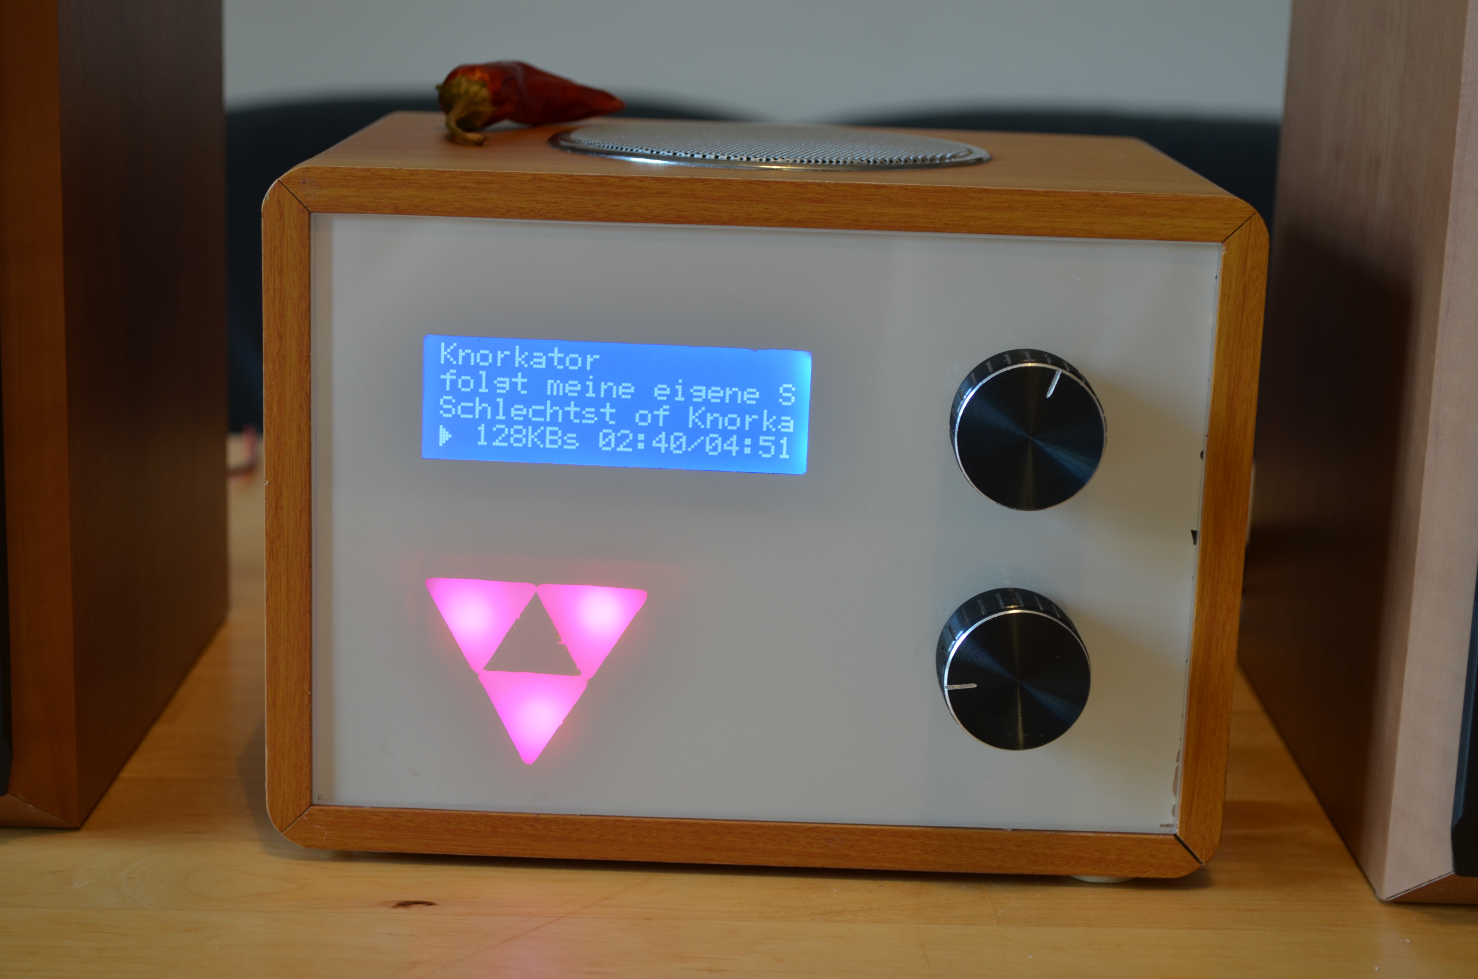
\includegraphics[width=0.5\textwidth]{images/front_3.png}
  \caption{Aktueller Prototyp}
  \label{fertig}
\end{figure}

\newpage 

Abbildung \ref{fertig} zeigt den \emph{Eulenfunk} Prototypen, welcher im
Zeitraum von drei Wochen im Rahmen des Hardwaresysteme Kür--Projekts
entstanden ist. Auf Vimeo\footnote{Eulenfunk Prototyp:
  \url{https://vimeo.com/171646691}} ist ein Video des aktuellen
Prototypen zu sehen.

\section{Verwendete Software}\label{verwendete-software}

Für die Entwicklung und Dokumentation wurden folgende \emph{GNU/Linux}
Tools verwendet:

\begin{itemize}
\tightlist
\item
  \emph{Pandoc/LaTeX} (Dokumentation)
\item
  \emph{Vim} (Softwareentwicklung)
\item
  \emph{Fritzing} (Schaltpläne).
\end{itemize}

\chapter{Motivation}\label{motivation}

\section{Private Situation}\label{private-situation}

Die Autoren dieses Projekts leben in einer Wohngemeinschaft zusammen.
Die Küche ist der Ort an welchem gemeinsam gekocht und gespeist wird.
Für eine angenehme Atmosphäre und als Nachrichten--Quelle sorgte in der
Küche früher ein Analog--Radio der Firma \emph{AEG}, welches aufgrund
der schlechten Empfangsqualität durch eine Kombination aus »alter
Stereoanlage«, »altem Raspberry Pi« und einem »alten Thinkpad X61t«
ersetzt wurde. In dieser Kombination fungierte die Stereoanlage als
Soundausgabe--Komponente, auf dem \emph{Raspberry Pi} lief der
Linux--basierte Player Volumio\footnote{Volumio:
  \url{https://volumio.org/}}, welcher mit dem Touchscreen des
\emph{Thinkpad x61t} über eine Weboberfläche gesteuert wurde. Diese
Kombination hat zwar funktioniert, jedoch war sie alles andere als
benutzerfreundlich, da zuerst die Stereoanlage und der Laptop
eingeschaltet werden mussten und eine WLAN--Verbindung zum
\emph{Raspberry Pi}--Player hergestellt werden musste. Diese Situation
weckte den Wunsch nach einer komfortableren Lösung, beispielsweise ein
Internetradio auf Basis des \emph{Raspberry Pi}.

\section{Kommerzielle Produkte}\label{kommerzielle-produkte}

Kommerzielle Anbieter von Internetradios gibt es wie Sand am Meer. Die
Preisspanne liegt hier zwischen \EUR{30} und mehreren hundert Euro. Der
Funktionsumfang sowie die Wiedergabequalität ist hier von Hersteller zu
Hersteller und zwischen den verschiedenen Preisklassen sehr
unterschiedlich. Einen aktuellen Überblick aus dem Jahr 2016 über
getestete Modelle gibt es beispielsweise online unter
\emph{bestendrei.de}\footnote{Test von Internetradios:
  \url{http://www.bestendrei.de/elektronik/internetradio/}}.

Das \emph{Problem} bei den kommerziellen Anbietern ist, dass man hier
jeweils an die vorgegebenen Funktionalitäten des Herstellers gebunden
ist. Bei einem Do--It--Yourself--Projekt auf Basis Freier Software
beziehungsweise eines freien Hardwaredesigns, hat man die Möglichkeit
alle gewünschten Funktionalitäten --- auch Features die von keinem
kommerziellen Anbieter unterstützt werden --- zu integrieren. Beispiele
für Funktionalitäten, welche bei kommerziellen Produkten nur schwer
beziehungsweise vereinzelt zu finden sind:

\begin{itemize}
\tightlist
\item
  Unterstützung bestimmter WLAN--Authentifizierungsstandards
\item
  Einhängen von benutzerdefinierten Dateifreigaben wie \emph{Samba},
  \emph{NFS}, \emph{SSHFS}
\item
  Unterstützung verschiedener \emph{lossy} und \emph{lossless} Formate
  \emph{OGG VORBIS}, \emph{FLAC}, u.a.
\item
  Integration verschiedener Dienste wie beispielsweise \emph{Spotify}
\item
  Benutzerdefinierte Anzeigemöglichkeiten (Uhrzeit, Wetter, et cetera.)
\end{itemize}

\chapter{Projektspezifikation}\label{projektspezifikation}

\section{Hardwareanforderungen}\label{hardwareanforderungen}

Das Radio soll dem Benutzer folgende Hardwarekonfigurationsmöglichkeiten
bieten:

\begin{itemize}
\tightlist
\item
  Anschluss passive Lautsprecher/Kopfhörer möglich
\item
  Lautstärkeregelung über Hardware möglich
\item
  Verwendung des internen Lautsprechers des alten Radios
\item
  Statusinformationen zum aktuellen Lied beispielsweise über ein LCD
\item
  LEDs als Statusanzeige und/oder als Visualisierungsvariante von
  Musik\footnote{Moodbar: \url{https://en.wikipedia.org/wiki/Moodbar}}
\item
  USB--Anschlussmöglichkeit für externe Datenträger
\end{itemize}

\section{Softwareanforderungen}\label{softwareanforderungen}

Die Software soll generisch gehalten werden um eine möglichst einfache
Erweiterbarkeit zu gewährleisten.

TODO Eule: Hier was zu Menü--Steuerung schrieben und Umfang?

\section{Optik-- und
Usability--Anforderungen}\label{optik-und-usabilityanforderungen}

Die Eingabe--Peripherie soll möglichst einfach gehalten werden, um eine
\emph{schöne} Produkt--Optik zu gewährleisten, dabei sollen folgende
Anforderungen erfüllt werden:

\begin{itemize}
\tightlist
\item
  Minimale sowie ansprechende Bedienelemente
\item
  Funktionales, zweckgebundenes \emph{Design}
\item
  \emph{Retro--Look}-Aussehen wünschenswert
\end{itemize}

Das \emph{Design} soll im Grunde \emph{minimalistisch} gehalten werden,
das heißt, es sollen aufgrund der Übersichtlichkeit nur so wenige
»Bedienelemente« wie nötig angebracht werden.

\chapter{Hardware}\label{hardware}

\section{Komponenten und Bauteile}\label{komponenten-und-bauteile}

Folgende Hardwarekomponenten oder Bauteile sind bereits vorhanden oder
müssen noch erworben werden:

\textbf{Vorhanden:}

\begin{itemize}
\tightlist
\item
  Altes Gehäuse AEG 4104 Küchenradio\footnote{AEG Küchenradio 4104:
    \url{https://www.amazon.de/AEG-MR-4104-Desgin-Uhrenradio-buche/dp/B000HD19W8}}
\item
  \emph{Raspberry Pi} aus dem Jahr 2012
\item
  LCD--Anzeige (Altbestände u. Arduino--Kit)
\item
  Kleinbauteile wie LEDs, Widerstände
\item
  USB--Hub für Anschluss von beispielsweise ext. Festplatte
\item
  USB--Soundkarte
\item
  Wi--Fi--Adapter
\item
  Netzteil (diverse 5V, 2mA)
\end{itemize}

\textbf{Muss noch erworben werden:}

\begin{itemize}
\tightlist
\item
  Audioverstärker
\item
  Drehimpulsregler
\item
  Kunststoffabdeckung für Front
\item
  Farbe (Lack)
\item
  Drehknöpfe für das Gehäuse
\end{itemize}

TODO Katze: Beschreibung an Diagrammpfeile

\begin{figure}[h!]
  \centering
  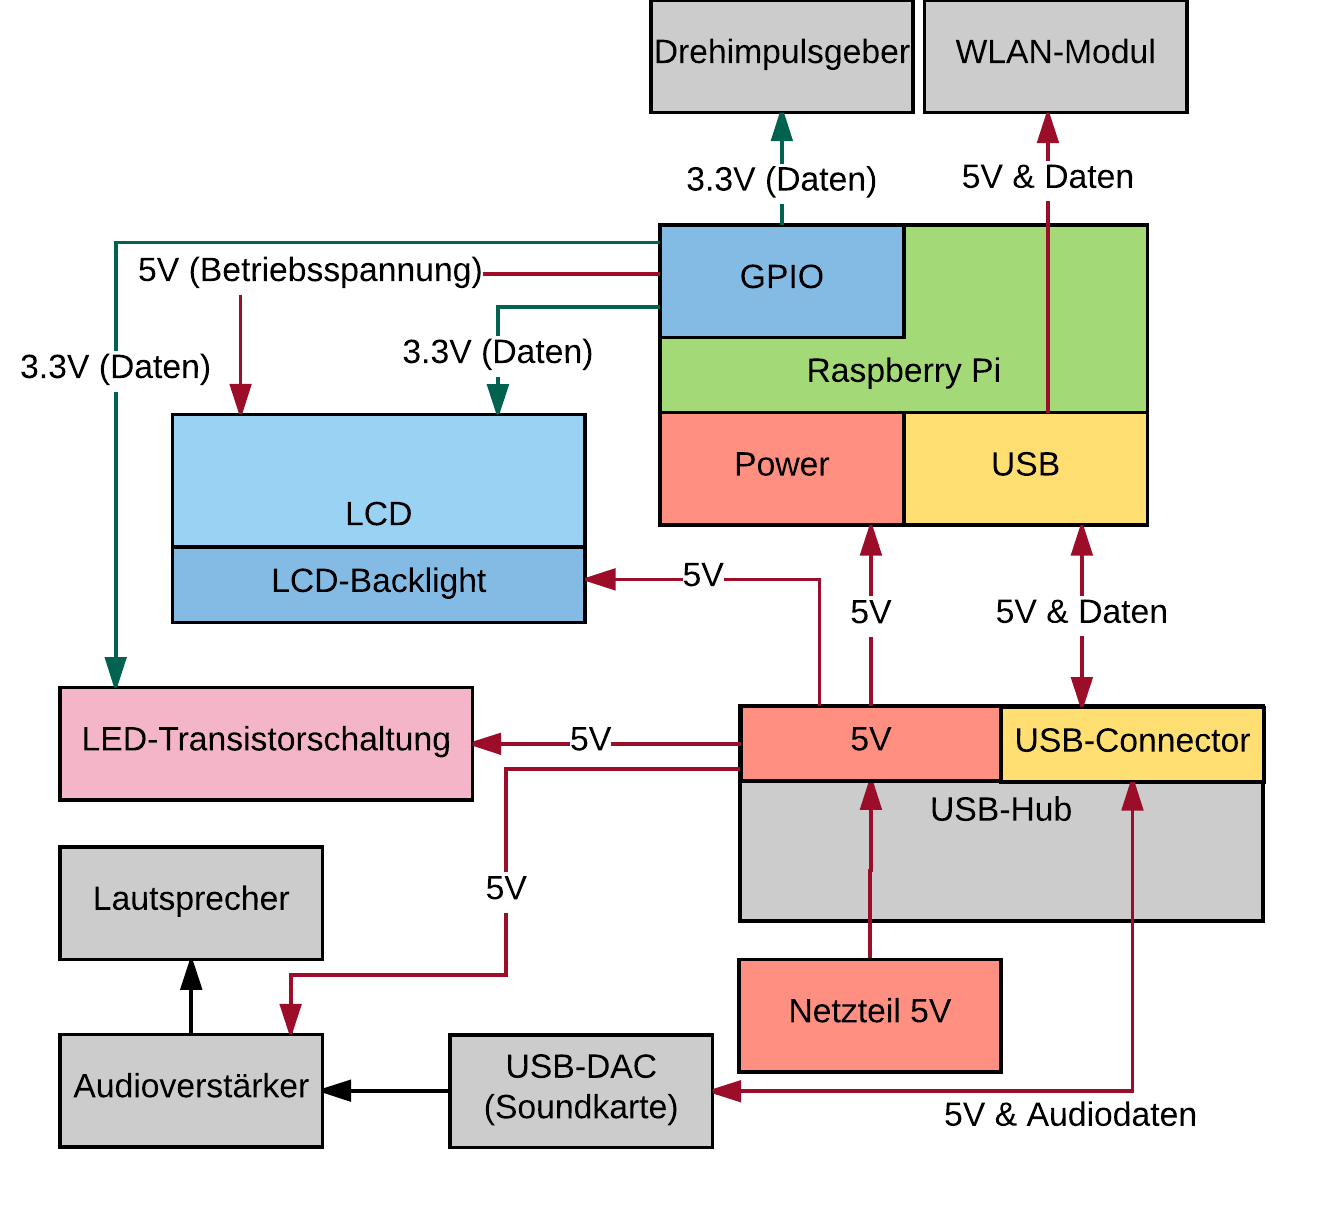
\includegraphics[width=0.7\textwidth]{images/uebersicht.png}
  \caption{Grobe Übersicht der verwendeten Komponenten im Zusammenspiel}
  \label{uebersicht}
\end{figure}

Abbildung \ref{uebersicht} zeigt eine konzeptuelle Übersichts des
Zusammenspiels der einzelnen Komponenten.

\section{Raspberry Pi}\label{raspberry-pi}

Der vorhandene \emph{Raspberry Pi} ist aus dem Jahr 2012. Die genaue
Hardware--Revision kann auf Linux unter \texttt{proc} ausgelesen werden,
siehe auch {[}1{]}, Seite 46:

\begin{Shaded}
\begin{Highlighting}[]

    \NormalTok{$ }\KeywordTok{cat} \NormalTok{/proc/cpuinfo }
    \KeywordTok{processor}       \NormalTok{: 0}
    \KeywordTok{model} \NormalTok{name      : ARMv6-compatible processor rev 7 (v6l)}
    \KeywordTok{BogoMIPS}        \NormalTok{: 697.95}
    \KeywordTok{Features}        \NormalTok{: half thumb fastmult vfp edsp java tls }
    \KeywordTok{CPU} \NormalTok{implementer : 0x41}
    \KeywordTok{CPU} \NormalTok{architecture: 7}
    \KeywordTok{CPU} \NormalTok{variant     : 0x0}
    \KeywordTok{CPU} \NormalTok{part        : 0xb76}
    \KeywordTok{CPU} \NormalTok{revision    : 7}

    \KeywordTok{Hardware}        \NormalTok{: BCM2708}
    \KeywordTok{Revision}        \NormalTok{: 0003}
    \KeywordTok{Serial}          \NormalTok{: 00000000b8b9a4c2}
\end{Highlighting}
\end{Shaded}

Laut Tabelle unter {[}1{]}, Seite 45 handelt es sich hierbei um das
Modell B Revision 1+ mit 256MB RAM.

Je nach Raspberry Revision sind die Pins teilweise unterschiedlich
belegt. Seit Modell B, Revision 2.0 ist noch zusätzlich der P5 Header
dazu gekommen. Abbildung \ref{gpio}\footnote{Bildquelle:
  \url{http://www.raspberrypi-spy.co.uk/2012/06/simple-guide-to-the-rpi-gpio-header-and-pins/\#prettyPhoto}}
zeigt die GPIO--Header des \emph{Raspberry Pi} Modell B Revision 1+.

\subsection{GPIO--Schnittstelle}\label{gpioschnittstelle}

\begin{figure}[h!]
  \centering
  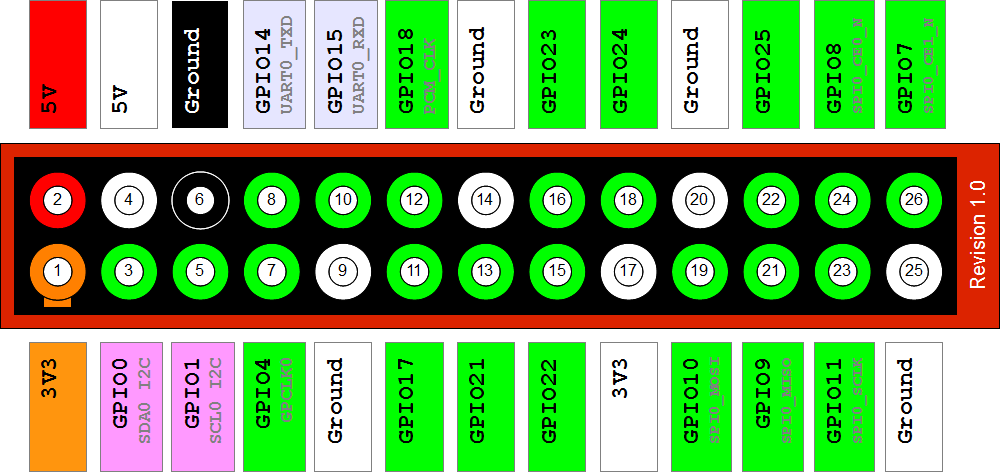
\includegraphics[width=0.7\textwidth]{images/gpio.png}
  \caption{GPIO-Header des Raspberry Pi Modell B Rev 1.0+}
  \label{gpio}
\end{figure}

\subsubsection{GPIO--Pinbelegung und
Funktionalität}\label{gpiopinbelegung-und-funktionalituxe4t}

Die GPIO--Pins des \emph{Raspberry Pi} haben eine Logikspannung von 3.3V
und sind pro GPIO--Pin mit max. 16mA belastbar. Der gesamte GPIO--Header
sollte mit nicht mehr als 50mA belastet werden, da es darüber hinaus zu
Hardwareschäden kommen kann (vgl. {[}1{]}, Seite 121 ff.).

Die \emph{Logik--Pegel} der GPIO--Pins sind beim \emph{Raspberry Pi} wie
folgt definiert {[}1{]}, Seite 129 ff.:

\begin{itemize}
\tightlist
\item
  \(\le\) 0,8V, input low
\item
  \(\ge\) 1,3V, input high
\end{itemize}

Die Ansteuerung von LEDs über GPIO erfolgt binär. Das heißt, dass die
LED entweder aus (low) oder an (high) sein kann.

In der »analogen« Welt ist es jedoch möglich eine LED über das Senken
der Spannung zu dimmen. Um ein Dimmen in der digitalen Welt zu erreichen
wird ein Modulationsverfahren angewandt, welches Pulsweitenmodulation
(PWM) heißt. Hierbei wird\ldots{}(Ref auf Software TODO: ELCH?) Unter
{[}2{]}, Seite 121 ff. und {[}3{]}, Seite 421 ff. finden sich weitere
Informationen.

Software PWM unter {[}4{]}, Seite 183 ff. zeigt beispielsweise eine 6\%
CPU--Last pro GPIO--Pin bei einer PWM--Softwareimplementierung. TODO:
ELCH?

\section{LCD--Anzeige}\label{lcdanzeige}

Um dem Benutzer --- beispielsweise Informationen über das aktuell
gespielte Lied --- anzeigen zu können, soll eine LCD--Anzeige verbaut
werden. In den privaten Altbeständen finden sich folgende drei
Hitachi--hd44780--kompatible Modelle:

\begin{itemize}
\tightlist
\item
  Blaues Display, 4x20 Zeichen, Bolymin BC2004A
\item
  Blaues Display, 2x16 Zeichen, Bolymin BC1602A
\item
  Grünes Display, 4x20 Zeichen, Dispalytech 204B
\end{itemize}

Für \emph{Eulenfunk} wurde das blaue 4x20 Display --- aufgrund der
größeren Anzeigefläche und Farbe --- gewählt.

\subsection{Anschlussmöglichkeiten}\label{anschlussmuxf6glichkeiten}

Eine LCD--Anzeige kann an den \emph{Raspberry Pi} auf verschiedene Art
und Weise angeschlossen werden. Anschlussmöglichkeiten für eine
LCD--Anzeige wären beispielsweise:

\begin{itemize}
\tightlist
\item
  GPIO direkt (parallel)
\item
  I2C--Bus (seriell)
\item
  SPI--Bus (seriell)
\end{itemize}

Die serielle Anschlussmöglichkeit bietet den Vorteil, dass weniger
Datenleitungen (GPIO--Pins) verwendet werden. Für den parallelen Betrieb
des Displays werden mindestens sechs GPIO--Pins benötigt, für den
seriellen Anschluss über I2C lediglich nur zwei.

Da für den seriellen Betrieb beispielsweise über den I2C--Bus
zusätzliche Hardware benötigt wird, wird die parallele Ansteuerung über
die GPIO--Pins bevorzugt. Weitere Informationen zum seriellen Betrieb
über I2C sind unter {[}5{]}, Seite 61, ff. zu finden.

\begin{figure}[h!]
  \centering
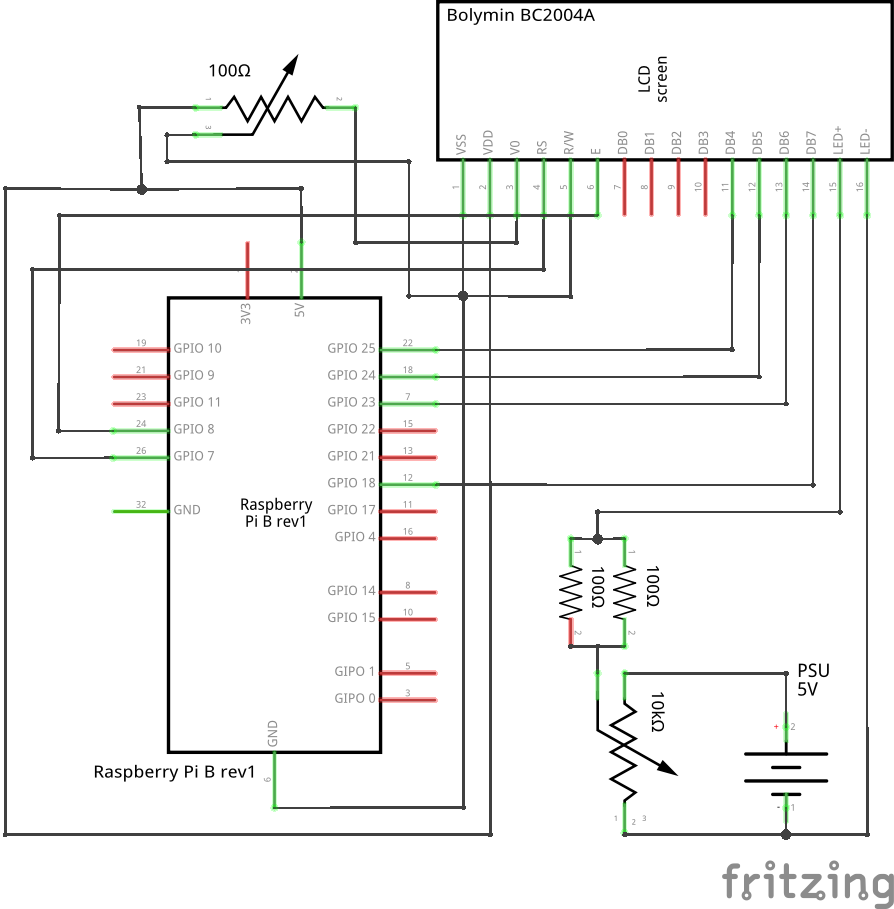
\includegraphics[width=0.7\textwidth]{images/lcdraspi.png}
  \caption{Verdrahtung von LCD im 4--Bit Modus und Raspberry Pi, alle hierzu benötigten
  Informationen sind im Datenblatt zu finden.}
  \label{lcd}
\end{figure}

Das Display arbeitet mit einer Logik--Spannung von 3.3V - 5V. Da die
GPIO--Pins jedoch eine High--Logik von 3,3V aufweisen, würde man hier in
der Regel einen Pegelwandler bei bidirektionaler Kommunikation und 5V
benötigen. Da aber auf das Display nur zugegriffen und die GPIO--Pins
nicht schreibend benutzt werden, kann ein Betrieb des Displays auch mit
5V erfolgen. Beim 3.3V Betrieb welcher laut Datenblatt\footnote{Datenblatt
  Bolymin BC2004A:
  \url{http://www.dema.net/pdf/bolymin/BC2004A-series_VER04.pdf}} auch
möglich sein soll, hatte das Display leider nur eine sehr schwachen
beziehungsweise unzureichenden Darstellungskontrast, weswegen der 5V
Betrieb gewählt wurde. Zudem wurde an \emph{Pin3} (LCD) ein
100\(\Omega\) Potentiometer hinzugefügt. Dies ermöglicht den Kontrast
variabel einzustellen.

Die Hintergrundbeleuchtung des Displays wurde direkt über ein
Potentiometer mit 2K\(\Omega\) an die 5V Spannungsversorgung
angeschlossen. Es wurde hier die direkte Speisung vom Netzteil gewählt,
um den GPIO--Header nicht unnötig zu belasten.

Laut Datenblatt kann die Hintergrundbeleuchtung entweder mit 3.4V ohne
Vorwiderstand oder mit 5V bei einem 27\(\Omega\) Widerstand betrieben
werden. Damit das Display beim herunter geregeltem Potentiometer keinen
Schaden nimmt, wurden zusätzlich zwei Widerstände mit 100\(\Omega\)
(parallel geschaltet = 50\(\Omega\)) zwischen Display und Potentiometer
gehängt.

Der resultierende Gesamtwiderstand ohne Potentiometer beträgt in diesem
Fall \(\approx\) 50 \(\Omega\):

\[  R_{ges} = \frac{R_1 \times R_2}{R_1 + R_2} = \frac{100\Omega \times 100\Omega}{100\Omega + 100\Omega} = 50\Omega \]

\section{Drehimpulsgeber}\label{drehimpulsgeber}

Um eine minimale Anzahl an Bedienelementen zu erhalten, wird bei
\emph{Eulenfunk} ein Drehimpulsgeber mit Schalter gewählt. Für erste
Testzwecke wurde von Herrn Schäferling ein \emph{ALPS STEC12E08}
bereitgestellt. Dieser wurde im Laufe der Entwicklung durch einen
\emph{ALPS STEC11B09}\footnote{Drehimpulsgeber ALPS STEC11B09:
  \url{https://www.reichelt.de/Drehimpulsgeber/STEC11B09/3/index.html?ACTION=3&GROUPID=3714&ARTICLE=73915}}
ersetzt, da dieser mittels Mutter und Schraube am Gehäuse besser
befestigt werden kann.

Der verwendete Drehimpulsgeber hat insgesamt fünf Anschlüsse. Zwei
Signalleitungen (A und B), zwei mal \emph{GND} (jeweils für Drehgeber
und Schalter) und einen Anschluss für den Schalter. Beim Drehen eines
Drehimpulsgebers wird ein Rechtecksignal generiert. Je nach Muster der
beiden Datensignale A oder B, kann entschieden werden ob es sich um eine
Rechts-- oder Linksdrehung handelt. Siehe {[}6{]}, Seite 361 ff. für
weitere Hintergrundinformationen zu Drehimpulsgeber.

Abbildung \ref{alps} zeigt den Anschluss des Drehimpulsgebers am
\emph{Raspberry Pi}.

\begin{figure}[h!]
  \centering
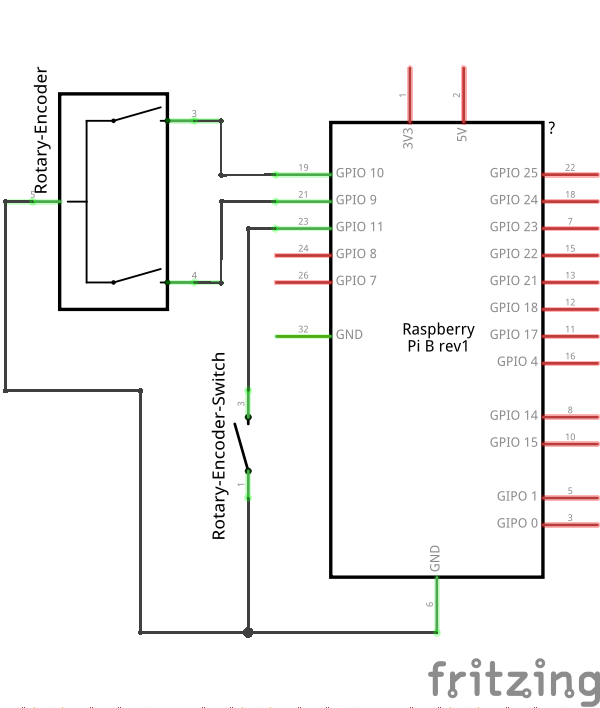
\includegraphics[width=0.8\textwidth]{images/rotary.png}
  \caption{Drehimpulsgeber--Anschluss an den Raspberry Pi, Abbildung zeigt
  Kombination aus Potentiometer und Schalter.}
  \label{alps}
\end{figure}

\section{Soundkarte}\label{soundkarte}

Die interne Soundkarte des \emph{Raspberry Pi} ist über eine triviale
Pulsweitenmodulation realisiert. Die einfache Schaltung soll hier laut
Internetquellen\footnote{Raspberry Pi onboard Sound:
  \url{http://www.crazy-audio.com/2013/11/quality-of-the-raspberry-pi-onboard-sound/}}eine
sehr niedrige Audioqualität bieten.

Aus diesem Grund wird bei \emph{Eulenfunk} auf das USB--Audio--Interface
\emph{BEHRINGER U-PHONO UFO202}\footnote{BEHRINGER U-PHONO UFO202 Audio
  Interface:
  \url{http://www.produktinfo.conrad.com/datenblaetter/1300000-1399999/001370864-an-01-de-BEHRINGER_UFO_202_AUDIOINTERFACE.pdf}}
(USB--Soundkarte) gesetzt.

\section{Audioverstärkermodul}\label{audioverstuxe4rkermodul}

Da eine Soundkarte in der Regel zu wenig Leistung hat, um einem
Lautsprecher »vernünftig« anzusteuern, wird ein Audioverstärker
benötigt. Da neben dem Anschluss von externen Lautsprechern auch eine
Lautstärkeregelung über ein Potentiometer erfolgen soll, ist die
Entscheidung einfachheitshalber auf ein Audioverstärker--Modul auf Basis
vom PAM8403\footnote{Verstärkermodul:
  \url{https://www.amazon.de/5V-Audioverstärker-Digitalendstufenmodul-Zweikanalige-Stereo-Verstärker-Potentiometer/dp/B01ELT81A6}}
Stereo-Verstärker mit Potentiometer gefallen. Eine
Do--It--Yourself--Alternative wäre ein Transistor--basierter
Audio--Verstärker, hier gibt es online diverse Bauanleitungen\footnote{Transistor--Verstärker:
  \url{http://www.newsdownload.co.uk/pages/RPiTransistorAudioAmp.html}}.

Das Audioverstärker--Modul hat folgende Anschlusspins:

\begin{itemize}
\tightlist
\item
  Left--In, Right--In, GND
\item
  5V+ und GND (Betriebsspannung)
\item
  Left--Side--Out (+), Left--Side--Out (-)
\item
  Right--Side--Out (+), Right--Side--Out (-)
\end{itemize}

Laut diverser Onlinequellen\footnote{PAM8403 Mono--Betrieb:
  \url{http://electronics.stackexchange.com/questions/95743/can-you-bridge-or-parallel-the-outputs-of-the-pam8403-amplifier}},
dürfen die Ausgänge für einen Mono--Betrieb eines auf dem
PAM8403--basierten Verstärkers nicht parallel geschaltet werden. Aus
diesem Grund kommt ein 4--poliger
\emph{EIN--EIN--Kippschalter}\footnote{Kippschalter 4--polig EIN--EIN:
  \url{http://www.reichelt.de/Kippschalter/MS-500P/3/index.html?&ACTION=3&LA=2&ARTICLE=13172&GROUPID=3275&artnr=MS+500P}}
zum Einsatz. So kann zwischen dem internen Lautsprecher (Mono--Betrieb)
und den externen Stereo Lautsprecher--Anschlüssen sauber per Hardware
hin und her geschaltet werden.

Damit im Mono--Betrieb nicht nur ein Kanal verwendet wird, ermöglicht
\emph{Eulenfunk} das Umschalten zwischen Mono-- und Stereo--Betrieb in
Software.

\section{LED--Transistorschaltung}\label{ledtransistorschaltung}

Die Ansteuerung einer LED mittels GPIO--Pin ist recht simpel. Sollen
jedoch mehrere LEDs angesteuert werden, so wird in der Regel pro LED ein
GPIO--Pin benötigt. LEDs sollten nie ohne Vorwiderstand an den
\emph{Raspberry Pi} angeschlossen werden, da durch den hohen Stromfluss
die LED beschädigt werden könnte. Weiterhin muss bei LEDs auch auf die
Polung geachtet werden, die abgeflachte Seite --- meist mit dem kürzerem
Beinchen -- ist in der Regel die Kathode (Minuspol). Abbildung \ref{led}
zeigt exemplarisch den Anschluss einer \emph{classic LED rot}\footnote{Datenblatt
  mit verschiedenen LED--Typen:
  \url{https://www.led-tech.de/de/5mm-LEDs_DB-4.pdf}}, mit einer
Flussspannung von \(U_{LED}\) \(\approx\) 2V, die mit einem Strom von
\(I_{LED}\) = 20 mA gespeist werden soll. Die Berechnung des
Vorwiderstandes erfolgt nach folgender Formel:

\[R_{LED} = \frac{U_{GPIO}-U_{LED}}{I_{LED}} = \frac{3.3V - 2V}{20mA}   \approx 65\Omega\]

\textbf{Hinweis:} Da ein GPIO--Pin aber mit nur max. 16mA belastet
werden sollte, sollte in unserem Beispiel durch 16mA anstatt 20mA
geteilt werden um den max. Stromfluss auf 16mA zu begrenzen. In diesem
Fall würden wir auf \(\approx\) 82\(\Omega\) kommen.

Da Widerstände meistens in fest vorgegebenen Größen vorhanden sind, kann
im Fall eines nicht exakt existierenden Widerstandswertes einfach der
nächsthöhere Widerstandswert genommen werden. Im Beispiel wird ein
\(100\Omega\) Widerstand verwendet.

Weitere Beispiele und Grundlagen zur Reihen-- und Parallelschaltung von
LEDs können online beispielsweise unter \emph{led-treiber.de}\footnote{Beispiele
  zur Ansteuerung von LEDs:
  \url{http://www.led-treiber.de/html/vorwiderstand.html}} eingesehen
werden.

\begin{figure}[h!]
  \centering
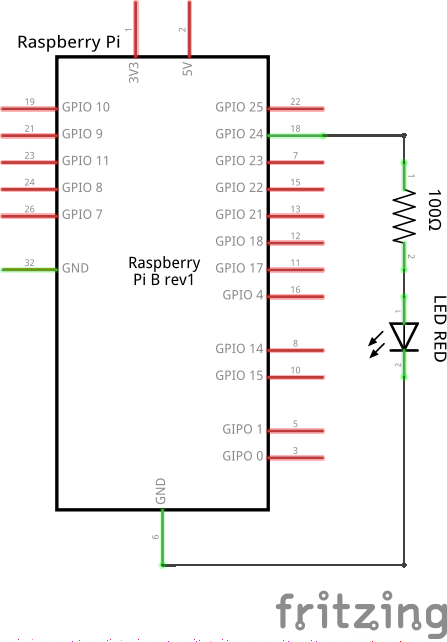
\includegraphics[width=0.5\textwidth]{images/led.png}
  \caption{Anschluss einer roten LED mit Vorwiderstand am Raspberry Pi GPIO--Pin}
  \label{led}
\end{figure}

Je nach Typ und Farbe ist der benötigte Strom um ein vielfaches höher
wie in unserem Beispiel. Die in \ref{led} abgebildete LED kann vom
GPIO--Pin nur einen max. Strom von 16 mA beziehen

In \emph{Eulenfunk} sollen mehrere intensiv leuchtende LEDs verbaut
werden. Da die GPIO--Pins in ihrer Leistung sehr begrenzt sind, würde es
sich anbieten eine externe Stromquelle zu verwenden. Um die Speisung
über eine externe Stromquelle zu ermöglichen, kann eine
Transistorschaltung verwendet werden (vgl. {[}7{]}, Seite 219 ff.).

Für die Transistorschaltung wurden von Herrn Schäferling NPN-- (BC547C)
und PNP--Transistoren (BC557C) bereitgestellt. Für den ersten Testaufbau
wurde der PNP--Transistor und eine RGB--LED\footnote{RGB-LED Common
  Cathode:
  \url{http://download.impolux.de/datasheet/LEDs/LED 0870 RGB 5mm klar 10000mcd.pdf}}
mit gemeinsamen Minuspol verwendet. Dabei ist aufgefallen, dass die LED
ständig geleuchtet hat. Eine kurze Recherche hat ergeben, dass der
Transistor permanent durchgeschaltet war, weil die Spannung an der Basis
(GPIO--Pin, 3,3V) geringer war als die Betriebsspannung für die LED
(5V).

Der zweite Testaufbau mit dem NPN--Transistor BC547C und einer
RGB--LED\footnote{RGB-LED Common Anode:
  \url{http://download.impolux.de/datasheet/LEDs/LED 09258 RGB 5mm klar 10000mcd_GP.pdf}}
mit gemeinsamen Pluspol hat das gewünschte Ergebnis geliefert.

Da der Hersteller für die von der Hochschule bereitgestellten
Transistoren unbekannt ist, wurden typische Durchschnittswerte für die
Dimensionierung der restlichen Bauteile verwendet.

Wie es aussieht sind die meisten BC547C Transistor--Typen für einen max.
Strom \(I_{CE}\)=100 mA konstruiert. Für die Berechnung des
Basis--Vorwiderstandes wird der Stromverstärkungsfaktor
\(h_{FE}\)\footnote{Stromverstärkungsfaktor:
  \url{http://www.learningaboutelectronics.com/Articles/What-is-hfe-of-a-transistor}}
benötigt. Je nach Hersteller variieren die Werte zwischen 200\footnote{Farichild
  Semiconductor:
  \url{https://www.fairchildsemi.com/datasheets/BC/BC547.pdf}} und
400\footnote{SEMTECH:
  \url{http://pdf1.alldatasheet.com/datasheet-pdf/view/42386/SEMTECH/BC547.html}}.
Da der maximale Laststrom \(I_{CE}\) pro Transistor 60 mA (3 LEDs je
max. 20mA) beträgt, sieht die Berechnung des Basisstroms --- bei einem
durchschnittlichem \(h_{FE}\) = 300 --- wie folgt aus:

\[I_{Basis} = \frac{I_{CE}}{h_{FE}} = \frac{0.06A}{300} \approx 200\mu A\]

Der BC547C Transistor benötigt eine durchschnittliche \(U_{BE}\) = 0,7V
zum Durchschalten. Die GPIO-Pins des \emph{Raspberry Pi} haben einen
Spannungspegel von 3.3V. Daraus ergibt sich folgende Berechnung des
Basis--Vorwiderstandes:

\[R_{Basis} = \frac{U_{GPIO} - U_{Basis}}{I_{Basis}} = \frac{3,3V - 0,7V}{200\mu A} = 13k\Omega \]

\begin{figure}[h!]
  \centering
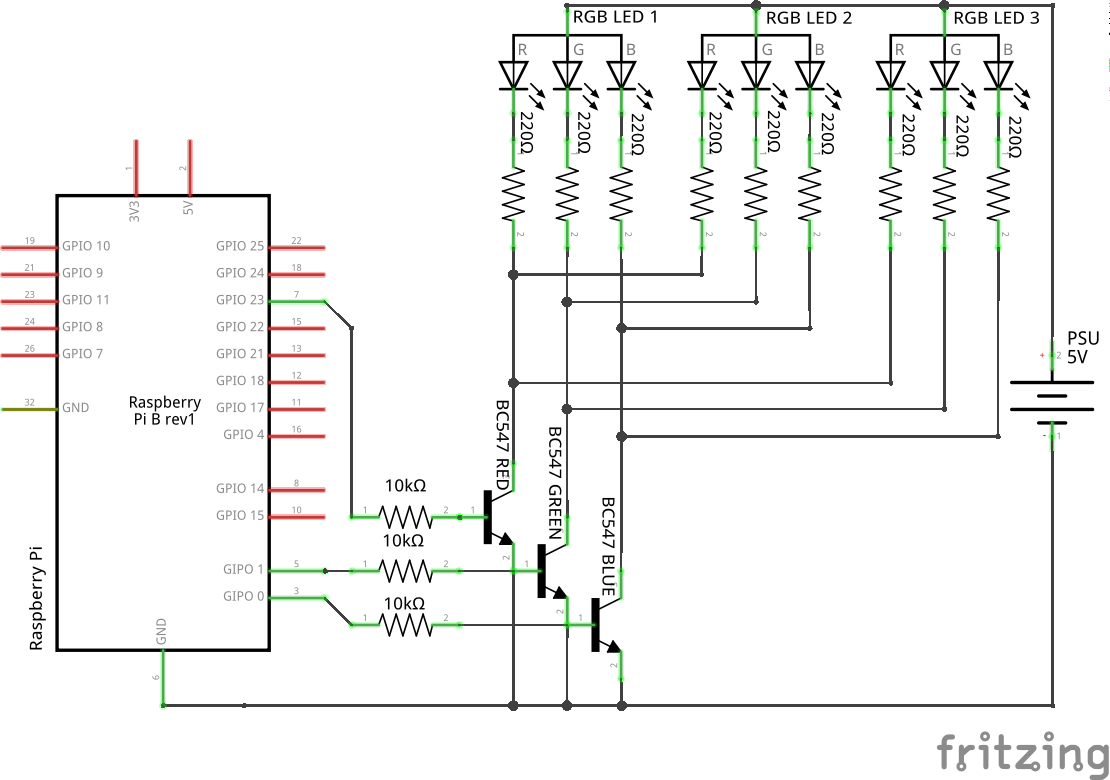
\includegraphics[width=0.9\textwidth]{images/transistorled.png}
  \caption{Transistor--RGB--LED Schaltung}
  \label{transled}
\end{figure}

Damit der Transistor jedoch \emph{sicher} durchschaltet, werden
Wiederstände mit \(10k \Omega\) verwendet. Die in Abbildung
\ref{transled} gelisteten LED--Vorwiderstände ergeben sich aufgrund der
verschiedenen Spannungen der unterschiedlichen Farben\footnote{RGB-LED
  Common Anode:
  \url{http://download.impolux.de/datasheet/LEDs/LED 09258 RGB 5mm klar 10000mcd_GP.pdf}}.
Die Berechnung für den Vorwiderstand pro LED schaut am Beispiel der
Farbe blau (\(U_{LED} = 3,15V, I_{LED} = 20mA\)) wie folgt aus:

\[R_{LED} = \frac{U_{Betriebsspannung} - U_{LED}}{I_{LED}} = \frac{5V - 3,15V}{20mA} =92.5 \approx 100\Omega\]

\section{USB--Hub und Netzteil}\label{usbhub-und-netzteil}

Der \emph{Raspberry Pi} hat in unserer Revision nur zwei
USB--Schnittstellen, diese sind bereits durch die Hardware--Komponenten
USB--DAC (Soundkarte) und das Wi--Fi--Modul belegt. Um den Anschluss
eines externen Datenträgers, auch mit größerer Last wie beispielsweise
einer Festplatte zu ermöglichen, wird ein aktiver USB--Hub benötigt.

Für diesen Einsatzzweck wird aus den Altbeständen ein \emph{LogiLink 4
Port USB 2.0 HUB}\footnote{LogiLink USB--Hub:
  \url{https://www.amazon.de/LogiLink-4-Port-Hub-Netzteil-schwarz/dp/B003ECC6O4}}
verwendet. Viele billig-Hubs arbeiten hier entgegen der
USB--Spezifikation und speisen den \emph{Raspberry Pi} zusätzlich über
die USB--Schnittstelle. Dieses Verhalten wurde bemerkt, als der
\emph{Raspberry Pi} ohne Power--Connector alleine nur mit der
USB--Verbindung zum USB--Hub bootete.

Bei der Speisung über die USB--Schnittstelle wird die interne
Sicherungsschaltung des \emph{Pi} umgangen, deswegen wird in der Regel
von einem Betrieb eines USB--Hub mit \emph{backfeed} abgeraten (vgl .
{[}8{]}, Seite 26 ff.). Für den Prototypen wird jedoch der genannte
USB--Hub und das dazugehörige Netzteil für den Betrieb von
\emph{Eulenfunk} verwendet. Das Netzteil ist für 5V bei max. 2A
ausgelegt.

\textbf{Nachtrag:} Die Speisung über das Netzteil des USB--Hubs ist
recht instabil. Bei Lastspitzen kommt es anscheinend zu
Störeinwirkungen, die sich auf die GPIO--Peripherie auswirken
(LCD--Anzeige rendert inkorrekt). Ein weiterer Punkt sind
Störfrequenzen, welche teilweise in Form von Störgeräuschen die
Audioausgabe überlagern (Hintergrundgeräusche beim Einschalten aller
LEDs). Insgesamt wurden drei Netzteile --- jeweils 5V, 2A
---ausprobiert. Von diesen war lediglich ein einziges als »akzeptabel«
einzustufen. Die restlichen zwei führen bei Lastspitzen zu Problemen
(Abstürze, fehlerhaftes Rendering auf Display, GPIO--Flips, et cetera).
Das \emph{backfeed} des USB--Hubs scheint die genannten Probleme
teilweise zu verstärken (vgl . {[}8{]}, Seite 27).

\section{Gehäuse}\label{gehuxe4use}

\subsection{Vorderseite}\label{vorderseite}

Abbildung \ref{ral} zeigt ein Muster der Gehäusefront--Farbe
hellelfenbeinweiß RAL 1015. Dieser Farbton wird für die Front verwendet,
um \emph{Eulenfunk} einen dezenten »Retro«--Look zu verpassen.

\begin{figure}[h!]
  \centering
  
\includegraphics[width=0.3\textwidth]{images/ral_soft.png}
  \caption{Muster RAL1015, hellelfenbeinweiß}
  \label{ral}
\end{figure}

Das Plexiglas für die Front wurde von der Firma \emph{ira-Kunststoffe}
in Schwarzenbach/Saale zugeschnitten. In der Plexiglasfront wurden mit
Hilfe von Herrn Schäferling zwei 5mm Löcher (Drehimpulsgeber,
Lautstärkeregler--Poti) gebohrt. Anschließend wurde die Plexiglas--Front
von der Innenseite lackiert\footnote{Buntlack, hellelfenbein:
  \url{http://www.obi.de/decom/product/OBI_Buntlack_Spray_Hellelfenbein_hochglaenzend_150_ml/3468725}},
hierbei wurden die Flächen für LCD und die drei LEDs abgelebt. Zudem
werden schwarze Knöpfe in Alu--Optik mit \(\diameter\) 30mm für den
Lautstärkeregler und den Drehimpulsgeber verwendet.

\subsection{Hinterseite}\label{hinterseite}

Für die Hinterseite wird die alte Abdeckung des AEG--Radios verwendet.
Diese musste teilweise leicht modifiziert werden. An dieser befinden
sich zwei Potis für Kontrastregelung und Hintergrundbeleuchtung des LCD,
eine USB--Female--Kabelpeitsche, zwei Cinch Stecker für externe
Lautsprecher und ein Kippschalter zum Umschalten zwischen internen und
externen Lautsprechern.

\section{Betriebssystem}\label{betriebssystem}

Mittlerweile gibt es für den \emph{Raspberry Pi} viele offiziell
zugeschnittene Betriebssysteme (vgl. {[}9{]}, Seite 29 ff., {[}10{]},
Seite 47 ff.). Bei den Linux--Distributionen ist \emph{Raspbian} eine
der bekanntesten Distribution -- welche auf \emph{Debian} basiert.
\emph{Raspbian} bringt ein komplettes Linux--basiertes System mit
grafischer Benutzeroberfläche mit sich.

Neben den unter {[}9{]}, Seite 29 ff. genannten Distributionen gibt es
mittlerweile auch Windows 10 IoT (Internet of Things) für den
\emph{Raspberry Pi}. Dieses speziell für den Embedded Bereich
ausgerichtete Windows benötigt jedoch eine ARMv7--CPU als
Mindestanforderung\footnote{Systemanforderungen:\url{http://raspberrypi.stackexchange.com/questions/39715/can-you-put-windows-10-iot-core-on-raspberry-pi-zero}},
was den »alten Raspberry« ausschließt. Außerdem wäre für uns eine
proprietäre Lösung ein K.O.--Kriterium, da diese alle Vorteile von
Freier Software zunichte machen würde.

\subsection{Wahl des Betriebssystem}\label{wahl-des-betriebssystem}

\emph{Arch Linux ARM}\footnote{Arch Linux ARM:
  \url{https://archlinuxarm.org/}} ist eine minimalistische und sehr
performante Linux--Distribution welche im Gegensatz zu \emph{Raspbian}
ohne Desktop--Umgebung geliefert wird (vgl. {[}11{]}, Seite 13 ff.)
Darüber hinaus ist \emph{Arch Linux} ein bekannter Vertreter von
Rolling--Release--Distributionen. Ein weiterer Vorteil für unseren
Einsatzzweck ist bei \emph{Arch Linux} das \emph{AUR} (Arch User
Repository)\footnote{Arch User Repository:
  \url{https://aur.archlinux.org/}}, dieses erlaubt es eigene Software
auf eine schnelle und unkomplizierte Weise der Allgemeinheit zur
Verfügung zu stellen.

\subsection{Einrichtung des
Grundsystems}\label{einrichtung-des-grundsystems}

Nach der Installation\footnote{Arch Linux Installation für Raspberry Pi:
  https://archlinuxarm.org/platforms/armv6/raspberry-pi\#installation}
und dem ersten Booten des Grundsystems muss die Netzwerk--Schnittstelle
konfiguriert werden. Arch Linux ARM bietet mit \emph{netctl} eine
Profil--basierte Konfigurationsmöglichkeit. Ein Profil kann über das
\emph{ncurses}--basierte Tool \texttt{wifi-menu} erstellt werden. In
unserem Fall wurde das Profil \texttt{wlan0-Phobos} erstellt.
Anschließend kann das erstellte Profil mit \emph{netctl} verwendet
werden.

\textbf{Auflistung der bekannten Profile}

\begin{Shaded}
\begin{Highlighting}[]
    \NormalTok{[}\KeywordTok{root@eulenfunk} \NormalTok{~]$ netctl list}
      \KeywordTok{eth0-static}
      \KeywordTok{wlan0-Phobos}
\end{Highlighting}
\end{Shaded}

\textbf{Aktivierung des gewünschten Profils}

\begin{Shaded}
\begin{Highlighting}[]
    \CommentTok{# Starten des gewünschten Profils}
    \NormalTok{[}\KeywordTok{root@eulenfunk} \NormalTok{~]$ netctl start wlan0-Phobos}
    \NormalTok{[}\KeywordTok{root@eulenfunk} \NormalTok{~]$ netctl list}
      \KeywordTok{eth0-static}
    \KeywordTok{*} \NormalTok{wlan0-Phobos}

    \CommentTok{# Profil über System-Reboot hinweg aktivieren }
    \NormalTok{[}\KeywordTok{root@eulenfunk} \NormalTok{~]$ netctl enable wlan0-Phobos}
\end{Highlighting}
\end{Shaded}

Nun verbindet sich der \emph{Raspberry Pi} nach dem Hochfahren jedes Mal
automatisch mit dem Profil \texttt{wlan0-Phobos}.

\subsection{Abspielsoftware}\label{abspielsoftware}

Für den Betrieb des Internetradios soll der MPD (Music--Player--Daemon)
verwendet werden, da \emph{Eulenfunk} auf einem eigens entwickeltem
MPD--Client basieren soll (mehr zur Eulenkfunk Software siehe Kapitel
Software). Andere Projekte greifen oft auf Abspielsoftware wie den
\emph{MOC} {[}9{]}, Seite 189 ff. oder \emph{mplayer} {[}7{]} Seite 638
ff. zu.

\begin{Shaded}
\begin{Highlighting}[]
    \CommentTok{# Installation des MPD}
    \NormalTok{[}\KeywordTok{root@eulenfunk} \NormalTok{~]$ pacman -Sy mpd mpc ncmpc}
\end{Highlighting}
\end{Shaded}

\chapter{Software}\label{software}

\section{Anforderungen}\label{anforderungen}

\begin{itemize}
\tightlist
\item
  Leichte integrierbarkeit mit anderen Anwendungen (lose Kopplung) TODO:
  Mehr.
\end{itemize}

\section{Softwarearchitektur}\label{softwarearchitektur}

Die Nachbaubarkeit vieler Bastelprojekte ist häufig durch die Software
recht eingeschränkt, da diese entweder nicht frei verfügbar ist oder zu
wenig generisch ist als dass man die Software leicht auf das Projekt
anpassen könnte. Meist handelt es sich dabei um ein einziges, großes
C--Programm oder ein eher unübersichtliches Python--Skript (TODO:
refs?). Aus diesem Grunde soll die Software für \emph{Eulenfunk} derart
modular aufgebaut sein, dass man einzelne Module problemlos auch auf
andere Projekte übertragbar sind und später eine leichte Erweiterbarkeit
gewährleistet ist. Damit auch andere die Software einsetzen können wird
sie unter die GPL in der Version 3 (TODO: ref) gestellt.

Zu diesem Zwecke ist die Software in zwei Hauptschichten unterteilt. Die
untere Schicht bilden dabei die \emph{Treiber}, welche die tatsächliche
Ansteuerung der Hardware erledigt. Dabei gibt es für jeden Teil der
Hardware einen eigene Treiber, im Falle von \emph{Eulenfunk} also ein
separates Programm für die LCD-Ansteuerung, das Setzen der LED Farbe und
dem Auslesen des oberen Rotary Switches.

Die Schicht darüber bilden einzelne Dienste (ingesamt fünf), die über
eine Netzwerkschnittstelle angesprochen werden und jeweils eine
Funktionalität des Radios umsetzen. So gibt es beispielsweise einen
Dienst der die Ansteuerung des LCD--Displays \emph{komfortabel} macht,
ein Dienst, der die LEDs passend zur Musik schaltet und ein Dienst der
automatisch eine Playlist aus der Musik auf angesteckten externen
Speichermedien erstellt. Die jeweiligen Dienste sprechen mit den
Treibern indem sie Daten auf \texttt{stdin} schreiben, bzw. Daten von
\texttt{stdout} lesen. Um die Dienste auf neue Projekte zu portieren ist
also nur eine Anpassung der Treiber notwendig.

Der Vorteil liegt dabei klar auf der Hand: Die lose Kopplung der
einzelnen Dienste erleichtert die Fehlersuche ungemein und macht eine
leichte Austauschbarkeit und Übertragbarkeit der Dienste in anderen
Projekte möglich. Stellt man beispielsweise fest, dass der Prozessor des
Radios voll ausgelastet ist, so kann man mit Tools wie \texttt{htop}
sehr einfach herausfinden welcher Dienst dafür verantwortlich ist.

\section{Überblick der einzelnen
Komponenten}\label{uxfcberblick-der-einzelnen-komponenten}

Ein Überblick über die existierenden Dienste liefert Abbildung
\ref{eulenfunk-services}.

\begin{figure}[h!]
  \centering
  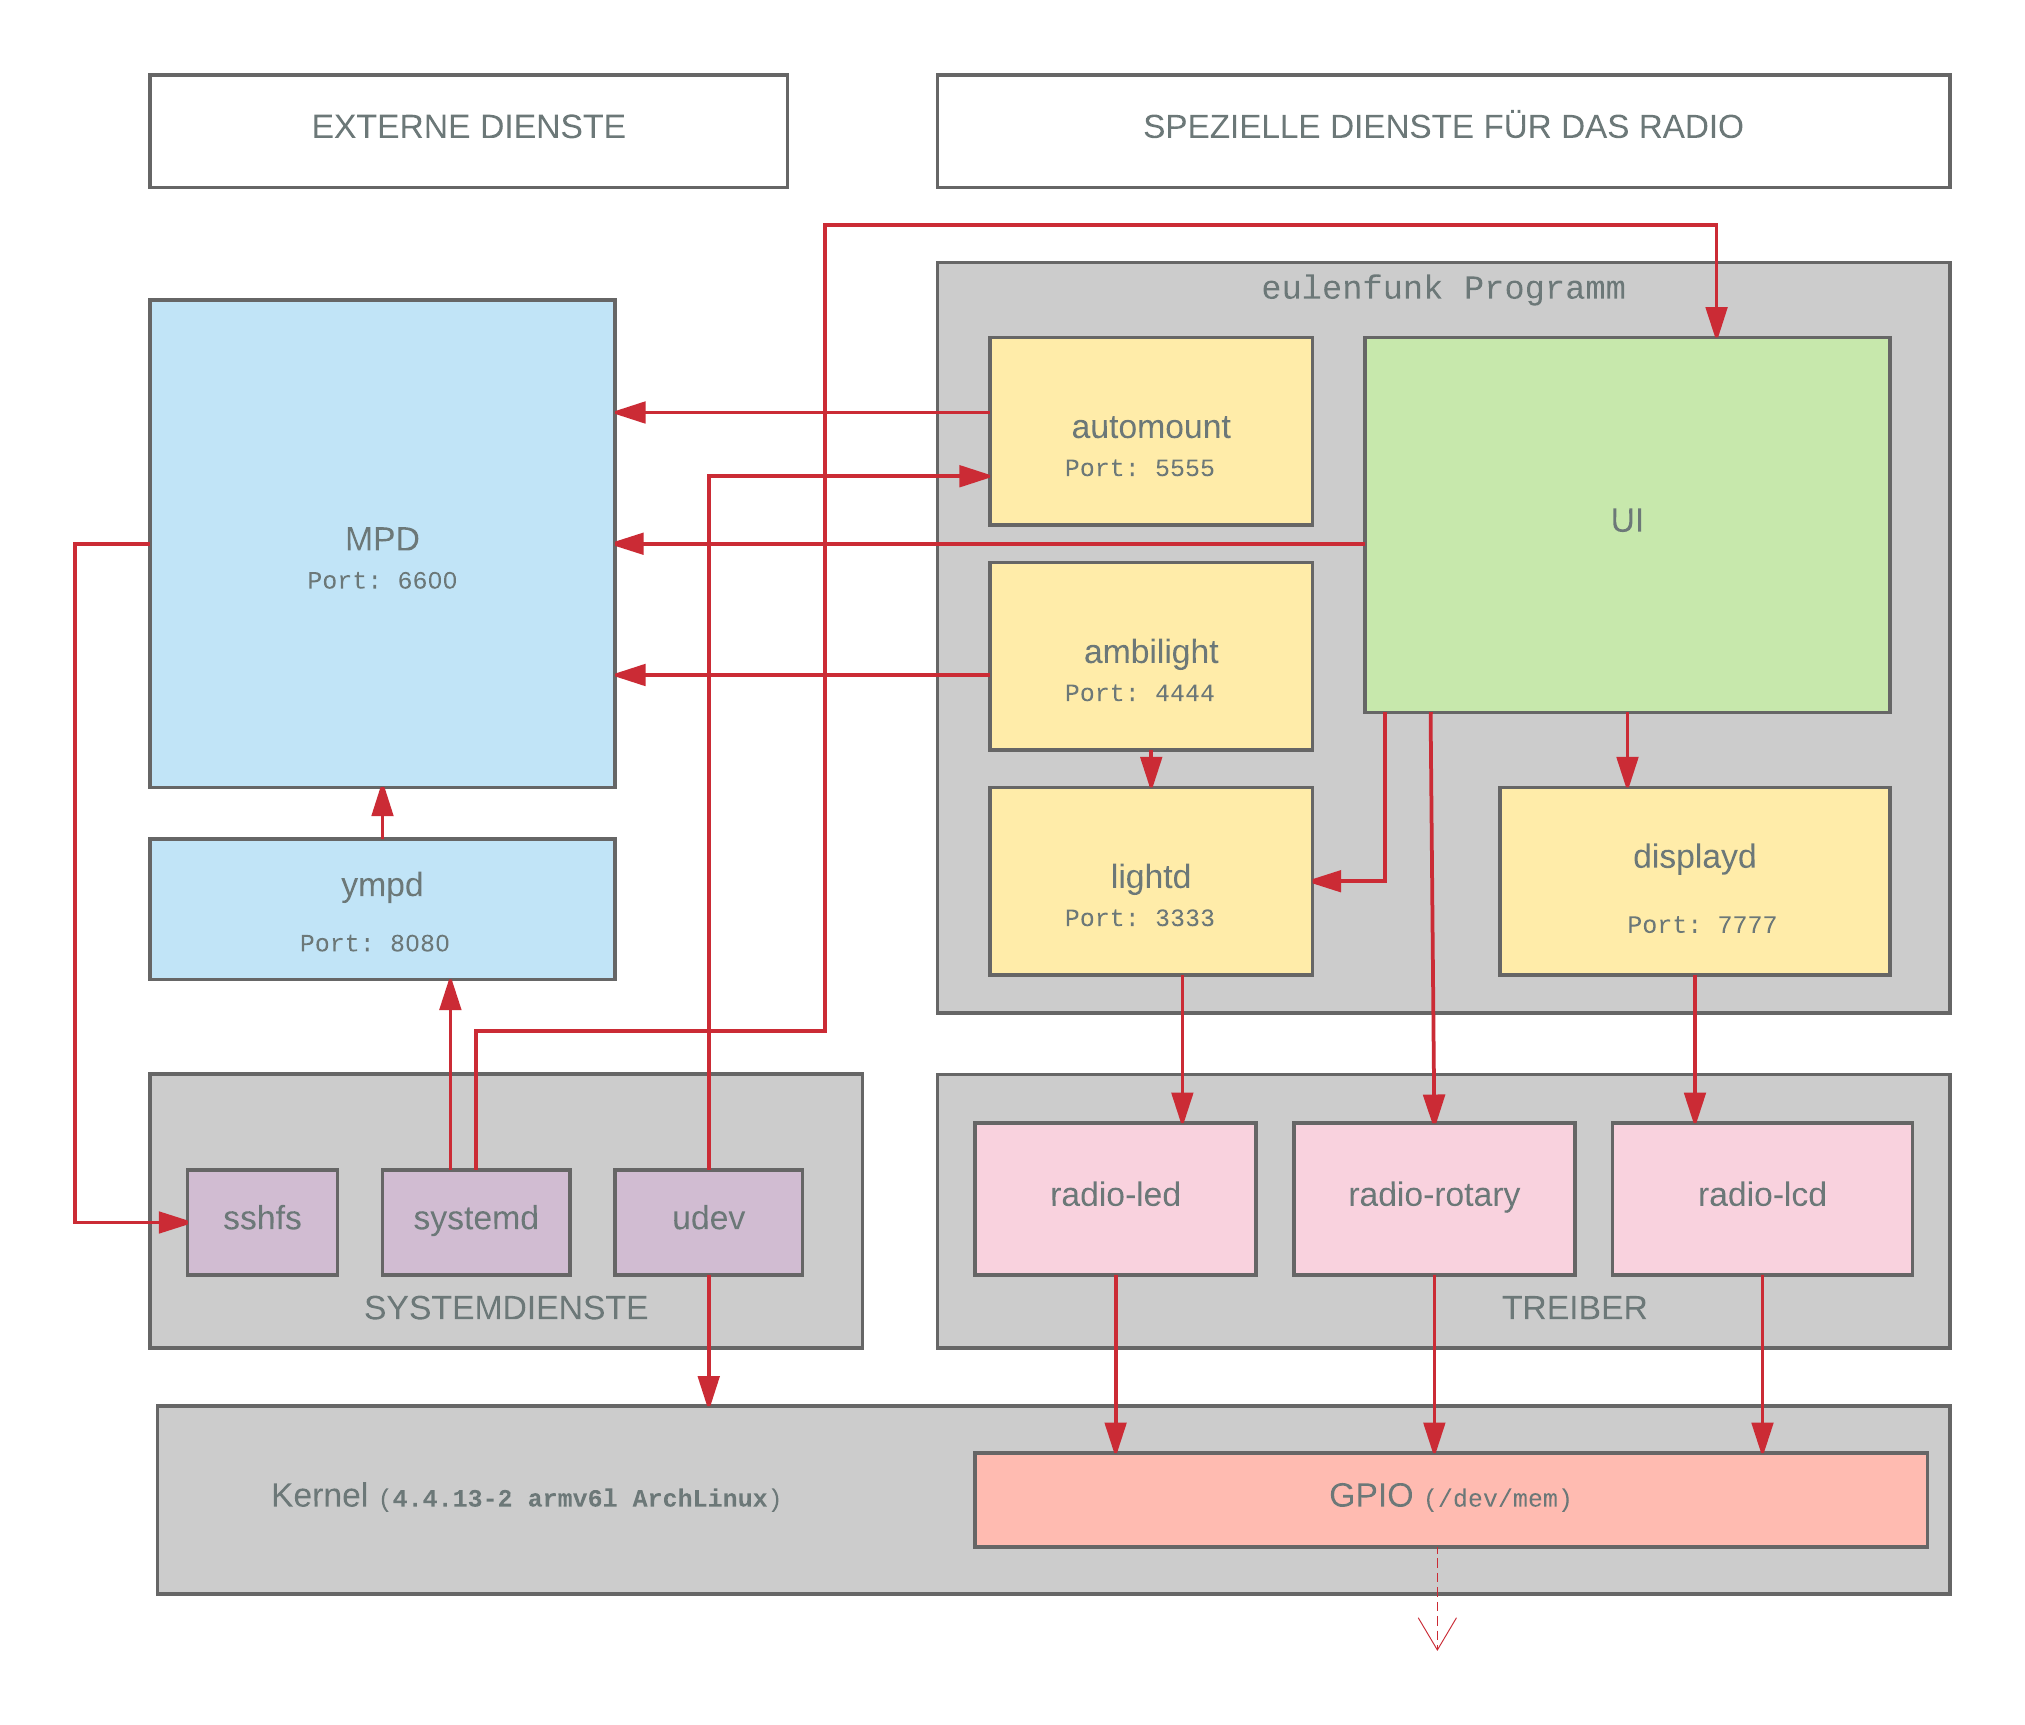
\includegraphics[width=1.0\textwidth]{images/eulenfunk-services.png}
  \caption{Übersicht über die Softwarelandschaft von Eulenfunk. Dienste mit
  einer Netzwerkschnittstelle sind durch den entsprechenden Port gekennzeichnet.}
  \label{eulenfunk-services}
\end{figure}

\subsection{Sprachwahl}\label{sprachwahl}

Die momentane Software ist in den Programmiersprachen \emph{C} und
\emph{Go} geschrieben. Dazu kommt lediglich ein Bash--Skript zum
Auslesen von Systeminformationen.

Die Ressourcen auf dem Raspberry Pi sind natürlich sehr limitiert,
weswegen sehr speicherhungrige Sprachen wie Java oder Ähnliches von
vornherein ausschieden. Obwohl Python nach Meinung des Autors eine
schöne Sprache ist und viele gute Bibliotheken für den Pi bietet, schied
es ebenfalls aus diesem Grund aus.

Ursprünglich war sogar geplant, alles in \emph{Go} zu schreiben. Leider
gibt es nur wenige Pakete für die GPIO Ansteuerung und auch keine
Bibliothek für Software--PWM. Zwar hätte man diese notfalls auch selbst
mittels \texttt{/sys/class/gpio/*} implementieren können, doch bietet
\emph{Go} leider keine native Möglichkeit mit Interrupts zu arbeiten.
Wie später beschrieben ist dies allerdings für den Treiber nötig, der
den Rotary Switch ausliest.

Für \emph{Go} sprechen wir ansonsten folgende Gründe:

\begin{itemize}
\tightlist
\item
  \textbf{Garbage collector:} Erleichtert die Entwicklung lang laufender
  Dienste.
\item
  \textbf{Hohe Grundperformanz:} Zwar erreicht diese nicht die
  Performanz von C, liegt aber zumindest in der selben Größenordnung
  (TODO: ref)
\item
  \textbf{Weitläufige Standardlibrary:} Kaum externe Bibliotheken
  notwendig.
\item
  \textbf{Schneller Kompiliervorgang:} Selbst große Anwendungen werden
  in wenigen Sekunden in eine statische Binärdatei ohne Abhängigkeiten
  übersetzt.
\item
  \textbf{Kross--Kompilierung:} Durch Setzen der \texttt{GOARCH}
  Umgebungsvariable kann problemlos auf einen
  x86-64--Entwicklungsrechner eine passende ARM--Binärdatei erzeugt
  werden.
\item
  \textbf{Eingebauter Scheduler:} Parallele und nebenläufige Anwendungen
  wie Netzwerkserver sind sehr einfach zu entwickeln.
\item
  Ein Kriterium war natürlich auch dass der Autor gute Erfahrung mit der
  Sprache hatte und \textbf{neugierig} war, ob sie auch für solche
  Bastelprojekte gut einsetzbar ist.
\end{itemize}

\texttt{C} ist hingegen für die Entwicklung der Treiber vor allem aus
diesen Gründen eine gute Wahl:**

\begin{itemize}
\tightlist
\item
  Programmierung mit \textbf{Interrupts} bequem und nativ möglich.
\item
  Höchste Performanz und geringer Speicherverbrauch.
\item
  Verfügbarkeit von wiringPi.
\end{itemize}

\subsection{Vorhandene
Softwarelibraries}\label{vorhandene-softwarelibraries}

Es folgt eine Liste der benutzten Bibliotheken:

\subsubsection{\texorpdfstring{\texttt{wiringPi}
(http://wiringpi.com)}{wiringPi (http://wiringpi.com)}}\label{wiringpi-httpwiringpi.com}

\texttt{wiringPi} ist eine Portierung der Arduino--\texttt{Wiring}
Bibliothek von Gordon Henderson auf den Raspberry Pi. Sie dient wie ihr
Arduino--Pendant zur leichten Steuerung der verfügbaren Hardware,
insbesondere der GPIO--Pins über \texttt{/dev/mem}. Daneben wird für den
LCD--Treiber auch die mitgelieferte LCD--Bibliothek genutzt. Für den
LED--Treiber wird zudem die softwarebasierte Pulsweitenmodulation
genutzt, allerdings in einer leicht veränderten Form.

\subsubsection{\texorpdfstring{\texttt{go-mpd}
(https://github.com/fhs/gompd)}{go-mpd (https://github.com/fhs/gompd)}}\label{go-mpd-httpsgithub.comfhsgompd}

Eine einfache MPD--Bibliothek, die wenig mehr als die meisten Kommandos
des MPD--Protokolls unterstützt.

TODO: ref (https://www.musicpd.org/doc/protocol/)

\subsubsection{\texorpdfstring{\texttt{go-colorful}
(github.com/lucasb-eyer/go-colorful)}{go-colorful (github.com/lucasb-eyer/go-colorful)}}\label{go-colorful-github.comlucasb-eyergo-colorful}

Eine Bibliothek um Farben in verschiedene Farbräume zu konvertieren. Der
Dienst der die LED passend zur Musik setzt nutzt diese Bibliothek um
RGB--Farbwerte in den HCL--Farbraum zu übersetzen. Dieser eignet sich
besser um saubere Übergänge zwischen zwei Farben zu berechnen und
Farbanpassungen vorzunehmen. Die genaue Funktionsweise wird weiter unten
beleuchtet (TODO: ref).

\subsubsection{cli
(github.com/urfave/cli)}\label{cli-github.comurfavecli}

Eine komfortable und reichhaltige Bibliothek um Kommandozeilenargumente
zu parsen. Unterstützt Subkommandos ähnlich wie \texttt{git}, welche
dann wiederum eigene Optionen oder weitere Subkommandos besitzen können.
Beide Features wurden extensiv eingesetzt, um alle in \emph{Go}
geschriebenen Dienste in einer Binärdatei mit konsistentem
Kommandozeileninterface zu vereinen.

\section{Treiber--Software}\label{treibersoftware}

In Summe gibt es momentan drei unterschiedliche Treiber. Sie finden sich
im \texttt{driver/} Unterverzeichnis\footnote{Siehe auf GitHub:
  \url{https://github.com/studentkittens/eulenfunk/tree/master/driver}}
der Software nebst einem passenden Makefile. Nach dem Kompilieren
entstehen drei Binärdateien, welche mit dem Präfix \texttt{radio-}
beginnen:

\begin{itemize}
\tightlist
\item
  \texttt{radio-led:} Setzt die Farbe des LED--Panels auf verschiedene
  Weise.
\item
  \texttt{radio-lcd:} Liest Befehle von \texttt{stdin} und setzt das
  Display entsprechend.
\item
  \texttt{radio-rotary:} Gibt Änderungen des Rotary Switches auf
  \texttt{stdout} aus.
\end{itemize}

Die genaue Funktionsweise dieser drei Programme wird im Folgenden näher
beleuchtet.

\subsection{\texorpdfstring{LED--Treiber
(\texttt{driver/led-driver.c})}{LED--Treiber (driver/led-driver.c)}}\label{ledtreiber-driverled-driver.c}

Der LED--Treiber dient zum Setzen eines RGB--Farbwerts. Jeder Kanal hat
den Wertebereich 0 bis 255. Die Hilfe des Programms zeigt die
verschiedenen Aufrufmöglichkeiten:

\begin{Shaded}
\begin{Highlighting}[]
\KeywordTok{usage}\NormalTok{:}
  \KeywordTok{radio-led} \NormalTok{on  ....... turn on LED (white)}
  \KeywordTok{radio-led} \NormalTok{off ....... turn off LED}
  \KeywordTok{radio-led} \NormalTok{cat ....... read rgb tuples from stdin}
  \KeywordTok{radio-led} \NormalTok{rgb  r g b  Set LED color to r,g,b}
  \KeywordTok{radio-led} \NormalTok{hex }\CommentTok{#RRGGBB Set LED color from hexstring}
  \KeywordTok{radio-led} \NormalTok{fade ...... Show a fade for debugging}
\end{Highlighting}
\end{Shaded}

Erklärung benötigt hierbei nur der \texttt{cat}--Modus, bei dem der
Treiber zeilenweise RGB--Farbtripel \texttt{stdin} liest und setzt.
Dieser Modus wird benutzt, um kontinuierlich Farben zu setzen ohne
ständig das Treiberprogramm neu zu starten.

\begin{figure}[h!]
  \centering
  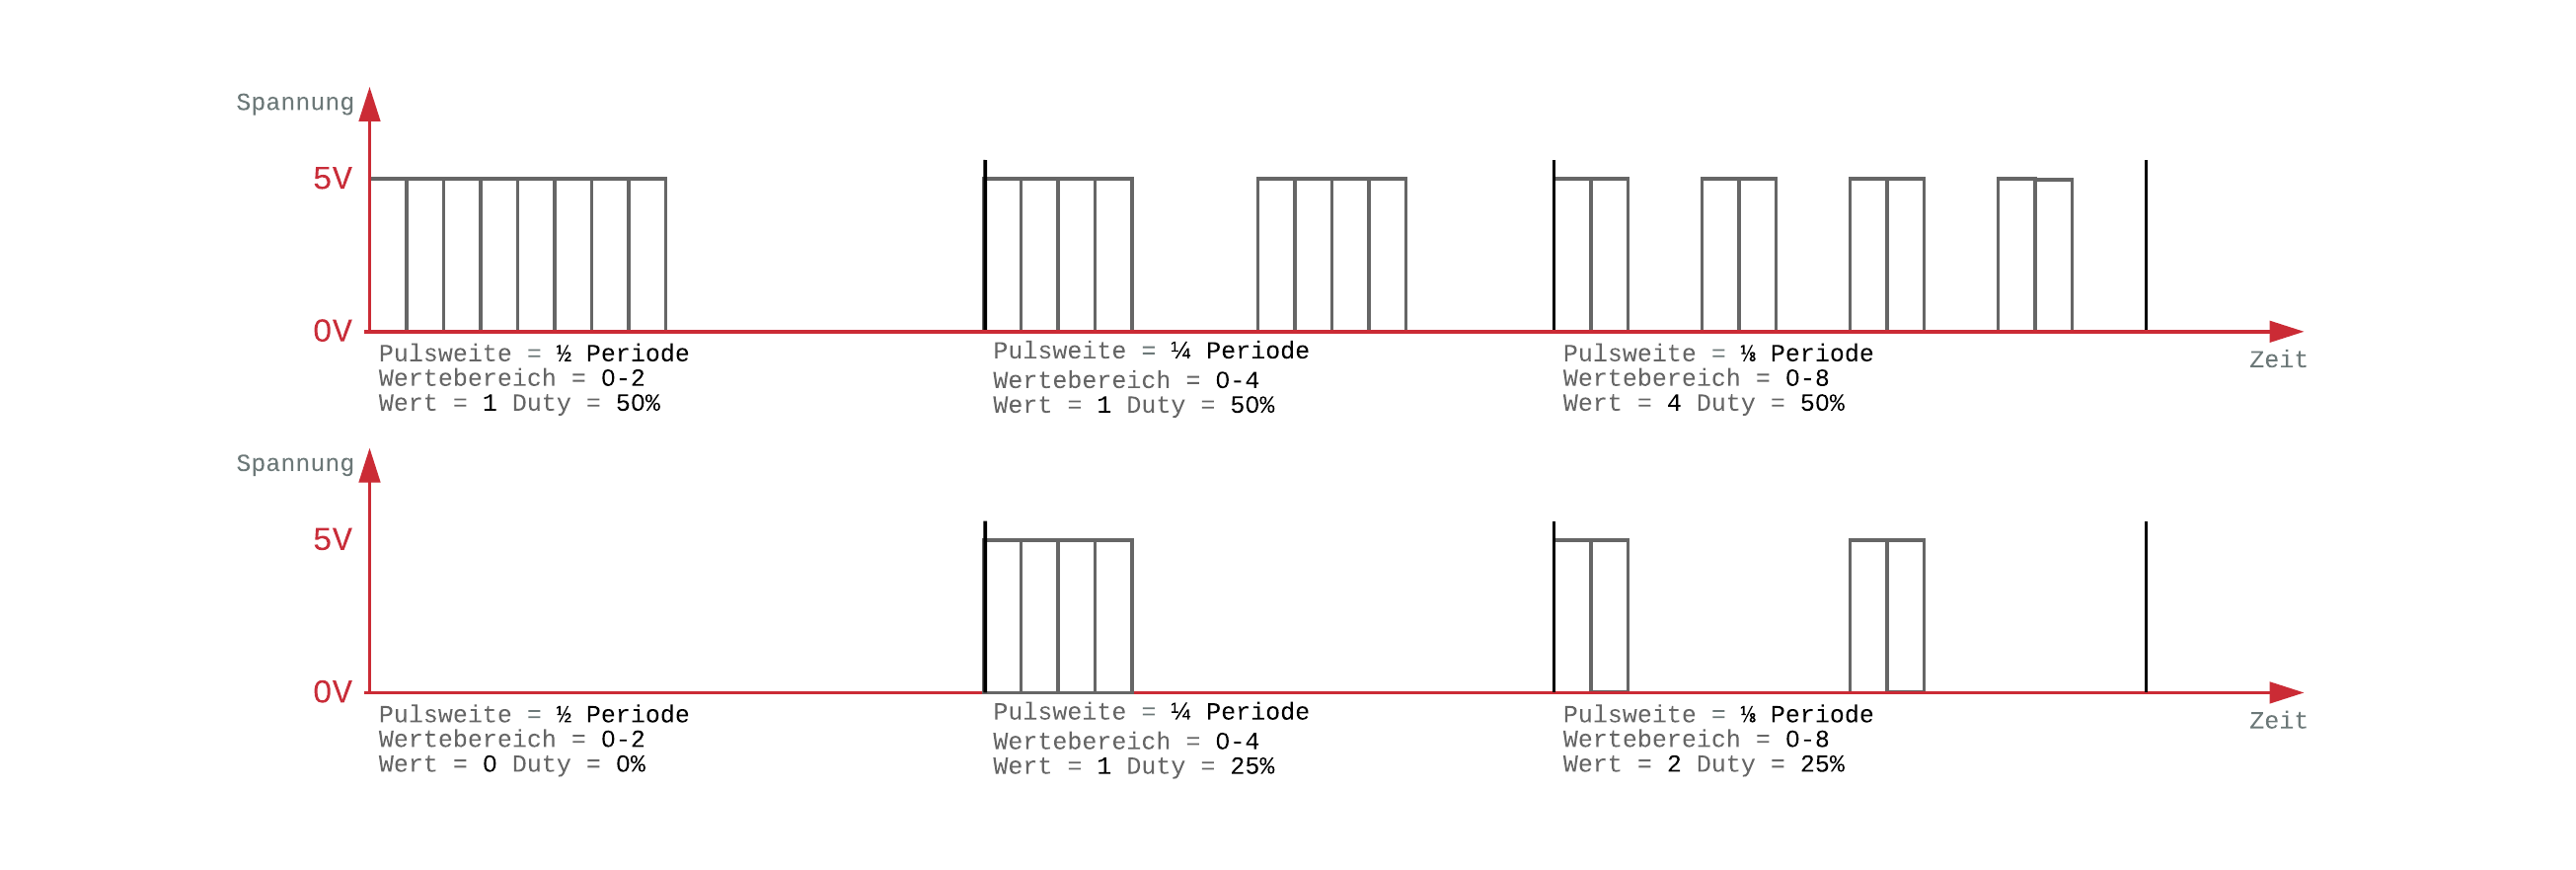
\includegraphics[width=1.0\textwidth]{images/eulenfunk-pwm.png}
  \caption{Grafische Darstellung der Pulsweitenmodulation}
  \label{eulenfunk-pwm}
\end{figure}

Da ein GPIO--Pin prinzipiell nur ein oder ausgeschaltet werden kann
verwenden wir Pulsweitenmodulation. Dabei macht man sich die träge Natur
des menschlichen Auges zu nutze indem man die LED sehr schnell
hintereinander ein und ausschaltet. Ist die LED dabei pro Ein- und
Ausschaltvorgang genauso lang hell wie dunkel so leuchtet die LED mit
etwa der Hälfte ihrer maximalen Leuchtstärke. Durch
Verlängerung/Verkürzung des eingeschalteten Zustands können so viele
verschiedene Helligkeitsstufen abgebildet werden. Siehe dazu auch
Abbildung \ref{eulenfunk-pwm}.

TODO: Diagramm/Text anpassen.

Da bei niedrigen Helligkeitswerten der ausgeschaltete Zustand besonders
lange gehalten wird, kann es dazu kommen dass ein flackerhafter Eindruck
entsteht, da man die ausgeschalteten Phasen als solche wahrnehmen kann.
Um dies zu verhindern muss eine ausreichende hohe Frequenz gewählt
werden.

Anders als ursprünglich angenommen, mussten wir feststellen dass die
GPIO Pins des Raspberry Pi (mit Ausnahme von Pin 18 (TODO: ref)) kein
hardwareseitiges PWM unterstützen. Aus diesem Grund mussten wir auf
softwareseitiges PWM zurückgreifen, um Farben mit mindestens 256
Abstufungen zu erhalten. Nach etwas Ausprobieren befanden wir die
\texttt{softPwm}--Bibliothek von \texttt{wiringPi} für tauglich (TODO:
ref).

Diese hat allerdings das Problem, dass eine hartkodierte Pulsweite von
100µs verwendet wird. Für die meisten Anwendungsfälle und den vom Autor
empfohlenen 100 Abstufungen ist das auch in Ordnung. Hundert
unterschiedliche Zustände waren nach kurzem Ausprobieren bei einem
weichen Farbübergang zu stark abgestuft.

\(T_{Periode} = 100\mu s\times 100= 10000\mu s = 0.01s\)

\(f = \frac{1}{T_{Periode}} = 100Hz\)

Optimal wären hier 256 unterschiedliche Zustände, um die volle 8-Bit
Farbtiefe auszunutzen. Daher mussten wir die entsprechende C--Datei
kopieren (GPL3--lizensiert) und manuell anpassen. Dabei haben wir die
Pulsweite auf 50µs herabgesetzt, was bei einer Spanne von 256 Werten
eine Frequenz von optisch akzeptablen 78Hz ergibt:

\(T_{Periode} = 50\mu s\times 256 = 12800\mu s = 0.0128s\)

\(f = \frac{1}{T_{Periode}} = 78.125Hz\)

Diese Frequenz scheint optisch ausreichend flackerfrei zu sein und
scheint die CPU nicht übermäßig stark zu beeinflussen (rund 2-3\% pro
Kanal).

Es besteht eine Verbindung zu einen früheren Bastelprojekt namens
\texttt{catlight}\footnote{\url{https://github.com/studentkittens/catlight}}
--- einer mehrfarbigen, in einem Gehäuse montierten LED die über USB
angesprochen werden kann. Genutzt wird diese zur Benachrichtigung bei
neuen E--Mails, Chat--Nachrichten und ähnlichem. Zu diesem Zwecke wurde
auch bereits damals ein Treiberprogramm entwickelt, welches das selbe
Bedienungskonzept wie \texttt{radio-led} hat. Dies war während der
Entwicklung von \emph{Eulenfunk} nützlich, da es die Entwicklung der
Dienste \texttt{ambilight} und \texttt{lightd} unabhängig von der
Radio--Hardware macht.

\subsection{\texorpdfstring{LCD--Treiber
(\texttt{driver/lcd-driver.c})}{LCD--Treiber (driver/lcd-driver.c)}}\label{lcdtreiber-driverlcd-driver.c}

\begin{Shaded}
\begin{Highlighting}[]
\KeywordTok{usage}\NormalTok{:}
  \KeywordTok{radio-lcd} \NormalTok{[print-charset [start [end]]]}
\end{Highlighting}
\end{Shaded}

Der LCD--Treiber setzt Bereiche des LCD--Displays auf einen gegebenen
Text. Beim Start leert er das Display und liest ähnlich wie
\texttt{radio-led\ cat} zeilenweise von \texttt{stdin} und entnimmt
diesen Zeilen die Information welchen Bereich des Displays gesetzt
werden soll. Das vom Treiber erwartete Zeilenformat ist dabei
\texttt{LINENO{[},OFFSET{]}\ TEXT...}, wobei \texttt{LINENO} die
gewünschte Zeilennummer als Dezimalzahl ist und der optionale
\texttt{OFFSET} der Index an dem geschrieben werden soll. Dahinter folgt
durch ein Leerzeichen getrennt beliebiger Text. Ist kein \texttt{OFFSET}
gegeben, so wird die ganze Zeile überschrieben und nötigenfalls mit
Leerzeichen aufgefüllt. Ist der Text länger als die Zeile wird der Text
abgeschnitten.

Der Treiber hält eine Matrix mit den aktuell gesetzten Zeichen und kann
daher ein erneutes Zeichnen einer Zelle im Display verhindern, indem es
das neue Zeichen mit dem Alten vergleicht. Unnötige Zeichenvorgänge
waren als störende Schlieren auf dem Display wahrnehmbar.

Zudem bietet der Treiber mit dem \texttt{print-charset} Argument die
Möglichkeit die auf dem Display verfügbaren Zeichen aufs selbige
auszugeben. Dazu stellt er jeweils 80 Zeichen da und wartetet einige
Sekunden bevor die nächsten 80 ausgegeben werden. Hat er alle 256
Zeichen ausgegeben beendet er sich. Optional kann man auch ein Start-
und End--Offset mitgeben, an dem er das Zeichnen anfangen soll.

Der Treiber unterstützt eine Reihe hardkodierter Spezialzeichen, welche
in der Menüführung und der UI zu benutzt werden. Das LCD--Display
unterstützt dabei 8 verschiedene \emph{Custom Chars}, welche mittels der
Codepoints 0-7 und 8-15 (wiederholt) setzbar sind. Momentan sind diese
auf folgende Glyphen gesetzt:

\begin{figure}[h!]
  \centering
  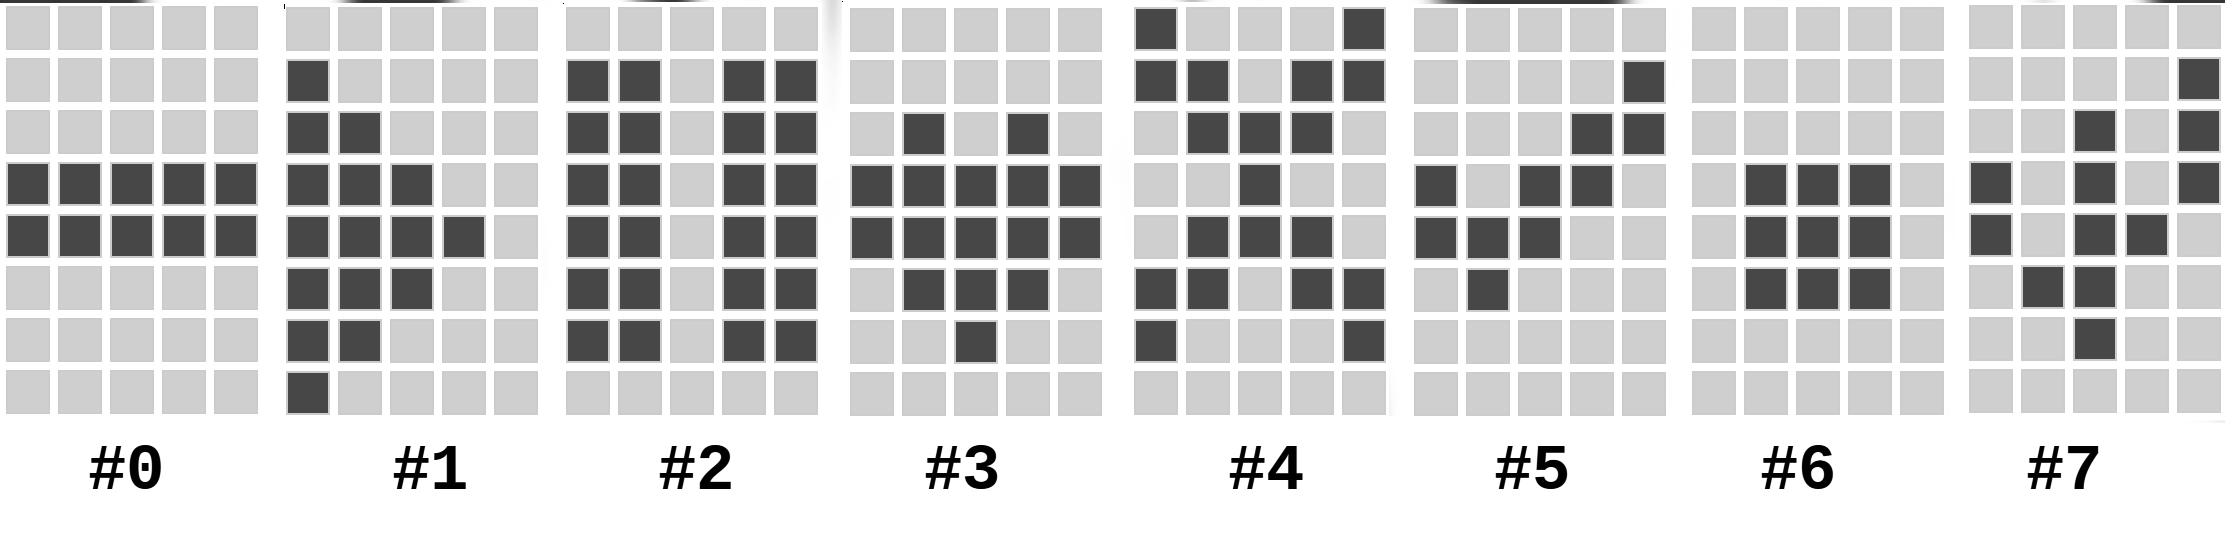
\includegraphics[width=1.0\textwidth]{images/symbols.png}
  \caption{}
  \label{eulenfunk-symbols}
\end{figure}

Die eigentliche Ansteuerung der Pins übernimmt dabei wieder die
\texttt{wiringPi}--Bibliothek, beziehungsweise dessen
LCD--Unterbibliothek (TODO: ref:
https://projects.drogon.net/raspberry-pi/wiringpi/lcd-library/). Diese
ist kompatibel mit dem Hitachi HD44780U und Nachbauten.

TODO:

\begin{itemize}
\tightlist
\item
  GPIO Anschluss?
\end{itemize}

\subsection{Drehimpulsgeber--Treiber}\label{drehimpulsgebertreiber}

\begin{itemize}
\tightlist
\item
  Prellung
\item
  ISR / kein printf
\item
  rotary encoder
\item
  http://theatticlight.net/posts/Reading-a-Rotary-Encoder-from-a-Raspberry-Pi/
\item
  grey code (buch zitieren)
\item
  button entprellen
\item
  \enquote{Polling} Mainloop
\item
  \enquote{Div by 3 hack}
\end{itemize}

\section{Service Software}\label{service-software}

\subsection{\texorpdfstring{\texttt{displayd} -- Der
Displayserver}{displayd -- Der Displayserver}}\label{displayd-der-displayserver}

\subsubsection{Einleitung}\label{einleitung}

Der Displayserver \texttt{displayd} kümmert sich um die Verwaltung der
Display--Inhalte. Er bietet eine höhere Abstraktionsschicht als der
vergleichsweise simple LCD--Treiber. Dabei bietet er die Abstraktion von
\emph{Zeilen}, \emph{Fenstern} und erleichtert dem Programmierer
Enkodierungsaufgaben indem es ein Subset von Unicode unterstützt. Eine
Zeile ist dabei eine beliebig langer utf8--enkodiertert Text ohne
Zeilenumbruch. Die Zeile kann dabei länger als das Display sein. In
diesem Fall wird die Zeile abgeschnitten oder scrollt je nach
Konfiguration mit einer bestimmten Geschwindigkeit durch. Ein Fenster
hingegen ist eine benannte Ansammlung von Zeilen. Auch ein Fenster kann
mehr Zeilen haben als das Display. Vom Nutzer kann der Fensterinhalt
dann vertikal verschoben werden. Es können mehrere Fenster verwaltet
werden, aktiv ist dabei aber nur ein ausgewähltes.

Die Idee diese Funktionalität in einem eigenen Daemon auszulagern, ist
vom Grafikstack in unixoiden Betriebssystemen inspiriert. Dabei kümmert
sich ebenfalls ein Displayserver um die Verwaltung der Inhalte (meist
\texttt{X.org} oder \texttt{Wayland}) indem er auf bestimmte Treiber
zurückgreift. Der Nutzer kann dann mittels eines festgelegten Protokolls
mit dem Displayserver sprechen und so unabhängig von der verwendeten
Rendering--Methode Inhalte darstellen. Da das Protokoll zwischen Client
und Displayserver meist trotzdem zu komplex ist, haben sich für diese
Aufgaben simple UI--Bibliotheken wie Xlib oder komplexere GTK+ und Qt
etabliert. Auch die Fenster--Metapher wurde dabei von den
Fenstermanagern übernommen.

Das Protokoll von \texttt{displayd} ist ein relativ simpel gehaltenes,
zeilenbasiertes Textprotokoll. Für den Zugriff auf dasselbige ist daher
wird auch keine UI--Bibliothek benötigt, lediglich einige Netzwerk und
Formatierungs--Hilfsfunktionen wurden implementiert (TODO: ref:
display/client.go). Basierend auf diesen Primitiven wurden aber auf
Clientseite Funktionalitäten wie Menü--»Widgets« implementiert, welche
die grafische Darstellung mit der Nutzereingabe verquicken.

Neben diesen Aufgaben löst \texttt{displayd} ein architektonisches
Problem: Wenn mehrere Anwendung versuchen auf das Display zu schreiben
käme ohne zentrale Instanz ein eher unleserliches Resultat dabei heraus.
Durch \texttt{displayd} können Anwendungen auf ein separates Fenster
schreiben, wovon jeweils nur eines aktiv angezeigt wird.

\subsubsection{Architektur}\label{architektur}

\begin{figure}[h!]
  \centering
  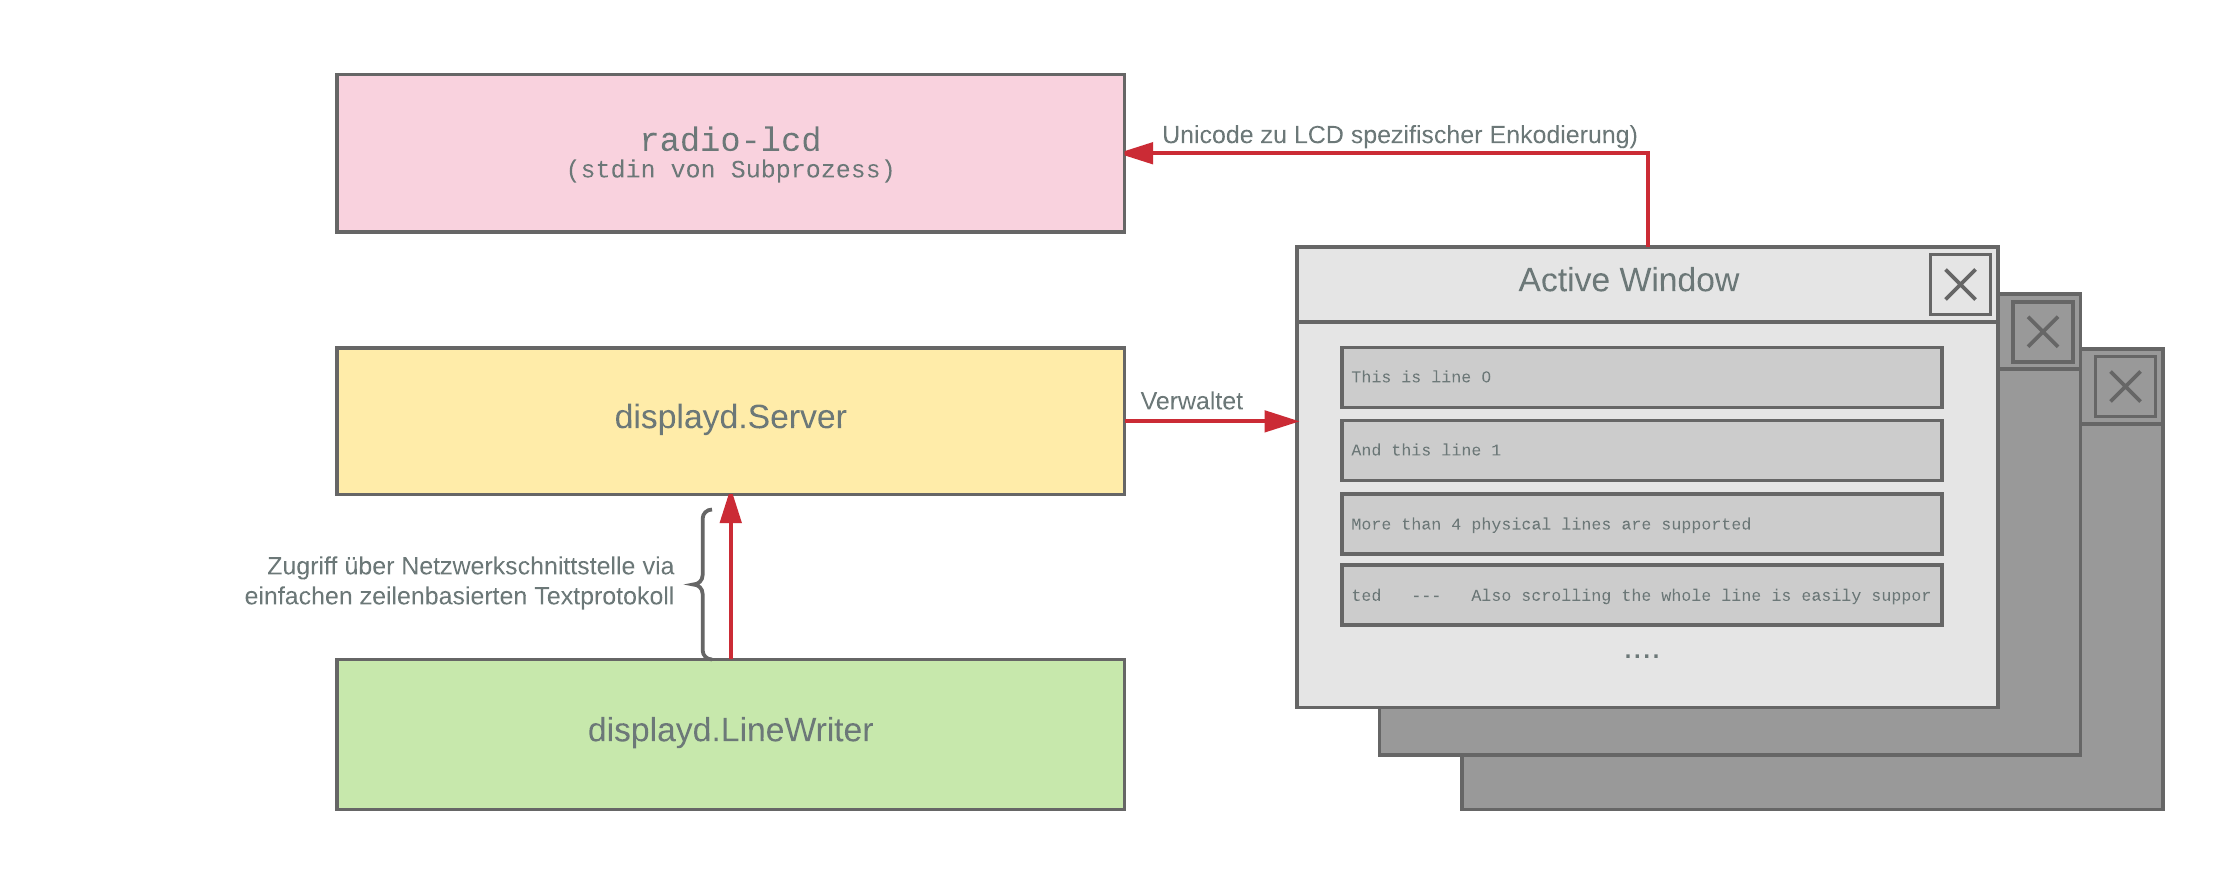
\includegraphics[width=1.0\textwidth]{images/eulenfunk-displayd.png}
  \caption{}
  \label{eulenfunk-displayd}
\end{figure}

Abbildung \ref{eulenfunk-displayd} zeigt die Architektur in der
Übersicht.

Nach dem Start kann man auf Port 7777 \texttt{displayd} mittels eines
simplen, zeilenbasierten Textprotokolls kontrollieren. Dabei werden die
folgenden Kommandos (mit Leerzeichen--getrennten Argumenten)
unterstützt:

\begin{verbatim}
switch <win>               -- Wechsle zum Fenster namens <win>.
line <win> <pos> <text>... -- Setze die Zeile <pos> im Fenster <win> zu <text>
scroll <win> <pos> <delay> -- Lässt Zeile <pos> in Fenster <win> mit der Geschwindigkeit <delay> scrollen.
move <win> <off>           -- Verschiebe Fenster <win> um <off> Zeilen nach unten.
truncate <win> <max>       -- Schneide Fenster <win> nach <max> Zeilen ab.
render                     -- Gebe aktuelles Fenster auf Verbindung aus.
close                      -- Schließt die aktuelle Verbindung.
quit                       -- Beendet Daemon und schließt Verbindung.

Dabei kann in die <Platzhalter> folgendes eingesetzt werden:

<win>:   Ein valider Fenstername (andernfalls wird ein neues Fenster mit diesen Namen angelegt)
<pos>:   Eine Zeilennummer, beginnend bei 0 für die erste Zeile.
<off>:   Ein Offset; 0 steht für keine Änderung; Kann negativ sein.
<max>:   Maximale Zeilenanzahl nach der das Fenster abgeschnitten wird.
<delay>: Zeitlicher Abstand zwischen zwei Scroll--Vorgängen.
         Siehe auch: https://golang.org/pkg/time/#ParseDuration
         Beispiel: 100ms
\end{verbatim}

Für die tatsächliche Anzeige nutzt \texttt{displayd} wie oben erwähnt
das Treiberprogramm \texttt{radio-lcd}. Dabei wird in periodischen
Abständen (momentan 150ms) das aktuelle Fenster auf den Treiber
geschrieben. Zukünftige Versionen sollen dabei intelligenter sein und
nur die aktuell geänderten Zeilen herausschreiben. Allerdings hat sich
herausgestellt, dass man mit mehreren scrollenden Zeilen bereits mit
diesen Ereignisbasierten Ansatz auf eine höhere Aktualisierungsrate
kommt als mit den statischen 150ms. Eine Art »VSync«, welches die
Aktualisierungsrate intelligent limitiert wäre hier in Zukunft
wünschenswert.

\subsubsection{Entwicklung}\label{entwicklung}

Da der Raspberry Pi nur bedingt als Entwicklungsplattform tauglich ist
(langsamer Compile/Run Zyklus), unterstützt \texttt{displayd} auch
Debugging--Möglichkeiten. Im Folgenden werden einige Möglichkeiten
gezeigt mit \texttt{displayd} zu interagieren, beziehungsweise Programme
zu untersuchen die \texttt{displayd} benutzen:

\begin{Shaded}
\begin{Highlighting}[]
\CommentTok{# Den display server starten; --no-encoding schaltet spezielles LCD encoding}
\CommentTok{# ab welches auf normalen Terminals zu Artifakten # führt. }
\NormalTok{$ }\KeywordTok{eulenfunk} \NormalTok{display server --no-encoding }\KeywordTok{&}

\CommentTok{# Gebe in kurzen Abständen das  "mpd" Fenster aus.}
\CommentTok{# (In separaten Terminal eingeben!)}
\NormalTok{$ }\KeywordTok{eulenfunk} \NormalTok{display --dump --update --window mpd}

\CommentTok{# Verbinde zu MPD und stelle aktuellen Status auf "mpd" Fenster dar.}
\NormalTok{$ }\KeywordTok{eulenfunk} \NormalTok{mpdinfo}
\CommentTok{# Auch nach Unterbrechung wird der zuletzt gesetzte Text weiterhin angezeigt:}
\NormalTok{$ }\KeywordTok{<CTRL-C>}
\CommentTok{# Änderungen sind auch möglich indem man direkt mit dem Daemon über telnet}
\CommentTok{# oder netcat spricht. Hier wird die erste Zeile überschrieben, das aktuelle}
\CommentTok{# Fenster angezeigt und dann die Verbindung geschlossen.}
\NormalTok{$ }\KeywordTok{telnet} \NormalTok{localhost 7777}
\KeywordTok{line} \NormalTok{mpd 0 Erste Zeile geändert!}
\KeywordTok{render}                        
\KeywordTok{close}
\end{Highlighting}
\end{Shaded}

\subsubsection{Enkodierung}\label{enkodierung}

Das LCD--Display unterstützt 8 bit pro Zeichen. Dabei sind die ersten
127 Zeichen weitesgehend deckungsgleich mit dem ASCII Standard.
Lediglich die Zeichen 0 bis 31 sind durch \emph{Custom Chars} und einige
zusätzliche Zeichen belegt. Dies ist insofern auch sinnvoll, da in
diesem Bereich bei ASCII Steuerzeichen definiert sind, die auf dem LCD
schlicht keinen Effekt hätten.

Die Zeichen 128 bis 255 sind vom Hersteller des Displays mit
verschiedenen Symbolen belegt worden, die keinem dem Autor bekannten
Encoding entsprechen. Da auch nach längerer Internetrecherche keine
passende Encoding--Tabelle gefunden werden konnte, wurde (in mühevoller
Handarbeit) eine Tabelle erstellt, die passende Unicode--Glyphen auf das
jeweilige Zeichen des Displays abbildet. Nicht erkannte utf8--Zeichen
werden als ein »?« gerendert anstatt Zeichen die mehrere Bytes zur
Enkodierung (wie » \$ \mu \$ «) als mehrere falsche Glyphen
darzustellen. So wird beispielsweise aus dem scharfen »ß« das Zeichen
223. Diese Konvertierung wird transparent von \texttt{displayd}
vorgenommen wodurch es möglich wird auch Musiktitel und ähnliches
(annäherend) korrekt darzustellen.

Abbildung \ref{eulenfunk-encoding} zeigt das erstellte Mapping zwischen
Unicode und LCD--Display. Folgende Seiten waren bei der Erstellung der
Tabelle hilfreich:

\begin{itemize}
\tightlist
\item
  http://www.amp-what.com (Suche mittels Keyword)
\item
  http://shapecatcher.com (Suche mittels Skizze)
\end{itemize}

\begin{figure}[h!]
  \centering
  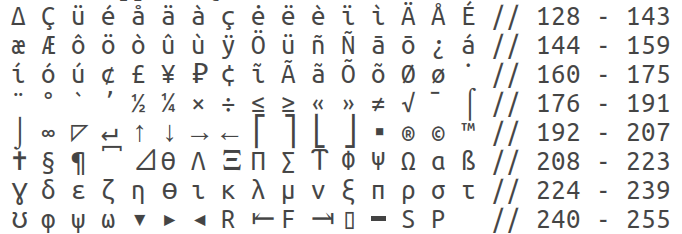
\includegraphics[width=1.0\textwidth]{images/encoding.png}
  \caption{Unicode Version der LCD--Glyphen}
  \label{eulenfunk-encoding}
\end{figure}

\subsection{\texorpdfstring{\texttt{lightd} -- Der
Effektserver}{lightd -- Der Effektserver}}\label{lightd-der-effektserver}

\texttt{lightd} ist ein relativ einfacher Service, dessen Hauptaufgabe
die Verwaltung auf den Zugriff auf die LED ist. Wollen mehrere Programme
die LED ansteuern, um beispielsweise einen sanften roten und grünen
Fade--Effekt zu realisieren so würde ohne Synchronisation zwangsläufig
ein zittrige Mischung beider Effekte entstehen.

Ursprünglich war \texttt{light} als \texttt{lockd} konzipiert, der den
Zugriff auf verschiedene Ressourcen verwalten kann. Da aber das Display
bereits von \texttt{displayd} synchronisiert wird und durchaus mehrere
Programme den Rotary Switch auslesen dürfen wurde diese etwa generellere
Idee wieder verworfen.

Die zweite Hauptaufgabe von \texttt{lightd} ist die Darstellung von
Farbeffekten auf der LED. Ursprünglich waren diese dafür gedacht um
beispielsweise beim Verlust der WLAN--Verbindung ein rotes Blinken
anzuzeigen. Momentan wird allerdings nur beim Herunterfahrend bzw.
Rebooten ein rotes bzw. oranges Blinken angezeigt. Folgende Effekte sind
also momentan als Möglichkeit zur Erweiterung zu begreifen:

\begin{itemize}
\tightlist
\item
  \texttt{blend:} Überblendung zwischen zwei Farben.
\item
  \texttt{flash:} Kurzes Aufblinken einer bestimmten Farbe.
\item
  \texttt{fade:} Lineare Interpolation von schwarz zu einer bestimmten
  Farbe und zurück.
\item
  \texttt{fire:} Kaminfeuerartiges Leuchten.
\end{itemize}

Wie andere Dienste wird auch \texttt{lightd} mittels einer
Netzwerkschnittstelle kontrolliert. Die mögliche Kommandoes sind dabei
wie folgt:

TODO: translate

\begin{verbatim}
// !lock      -- Try to acquire lock or block until available.
// !unlock    -- Give back lock.
// !close     -- Close the connection.
// <effect>   -- Lines starting without ! are parsed as effect spec.
//
// <effect> can be one of the following:
//
//   {<r>,<g>,<b>}
//   blend{<src-color>|<dst-color>|<duration>}
//   flash{<duration>|<color>|<repeat>}
//   fire{<duration>|<color>|<repeat>}
//   fade{<duration>|<color>|<repeat>}
//
// where <*-color> can be:
//
//   {<r>,<g>,<b>}
//
// and where <duration> is something time.ParseDuration() understands.
// <repeat> is a simple integer.
//
// Examples:
//
//   {255,0,255}                     -- The world needs more solid pink.
//   fire{1ms|{255,255,255}|0}       -- Warm fire effect.
//   blend{{255,0,0}|{0,255,0}|2s}   -- Blend from red to green.
\end{verbatim}

\subsection{\texorpdfstring{\texttt{ambilightd} -- Optische
Musikuntermalung}{ambilightd -- Optische Musikuntermalung}}\label{ambilightd-optische-musikuntermalung}

Ein »Gimmick« von \emph{Eulenfunk} ist es, dass die LED entsprechend zur
momentan spielenden Musik eingefärbt wird. Hier erklärt sich auch der
Name dieses Dienstes: \emph{Ambilight} (TODO: ref) bezeichnet eigentlich
eine von Phillips entwickelte Technologie, um an einem Fernseher
angebrachte LEDs passend zum momentanen Bildinhalt einzufärben. Hierher
kommt auch die ursprüngliche Idee dies auf Musik umzumünzen.

Um aus den momentan spielenden Audiosamples eine Farbe abzuleiten gibt
es einige Möglichkeiten. (TODO: hier HW schaltung etc. von oben
aufgreifen). Eine große Einschränkung bildet hierbei allerdings die sehr
begrenzte Rechenleistung des Raspberry Pi. Daher haben wir für eine
Variante entschieden, bei der die Farbwerte vorberechnet werden. Das
hast den offensichtlichen Nachteil, dass man für Radiostreams kein
Ambientlicht anzeigen kann. Andererseits möchte man das bei
Nachrichtensendung und Diskussionsrunden vermutlich auch nicht.

Zur Vorberechnung nutzen wir dabei das \texttt{moodbar} Programm (TODO:
http://cratoo.de/amarok/ismir-crc.pdf). Diese analysiert mit Hilfe des
GStreamer--Frameworks (TODO: ref) eine Audiodatei in einem
gebräuchlichen Format und zerlegt diese in 1000 Einzelteile. Kurz
erklärt\footnote{Der eigentliche Algorithmus ist komplexer und wird im
  referenzierten Paper beschrieben.} wird für jedes dieser Teile ein
Farbwert berechnet, wobei niedrige Frequenzen zu roten Farbtönen werden,
mittlere Frequenzen zu Grüntönen und hohe Frequenzen zu blauen Tönen
werden. Die so gesammelten Farbwerte werden dann in einer \texttt{.mood}
Datei gespeichert, welche aus 1000 RGB--Tripeln à 3 Byte (1 Byte pro
Farbkanal) bestehen. Ein visualisiertes Beispiel für eine Moodbar kann
man in Abbildung \ref{queen-moodbar} sehen.

\begin{figure}[h!]
  \centering
  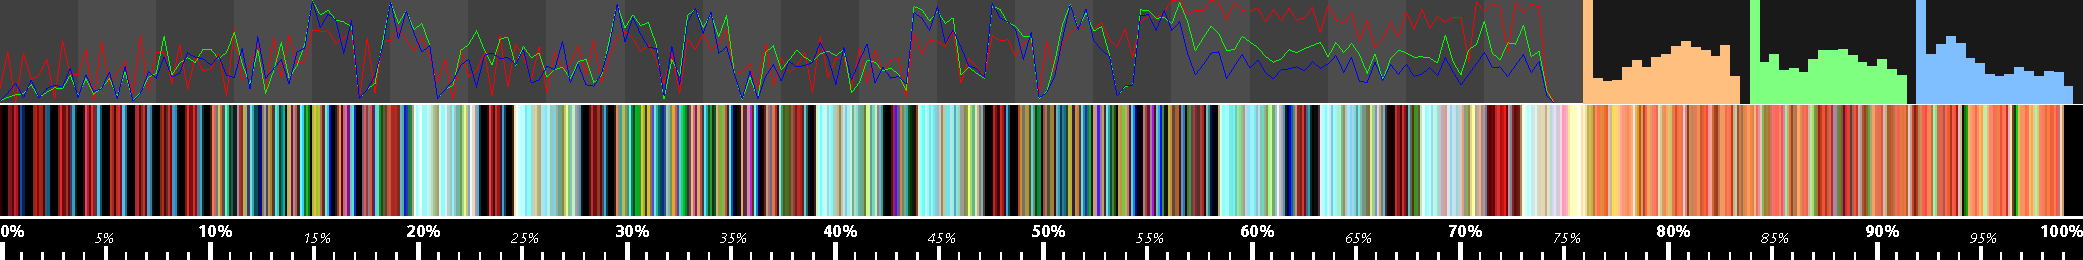
\includegraphics[width=1.0\textwidth]{images/we-will-rock-you-mood.pdf}
  \caption{Moodbar--Visualisierung des Liedes »We will rock you« von »Queen«.
  Das Fußstapfen und Klatschen am Anfang ist gut erkennbar.
  Die Visualisierung wurde mit einem Python--Skript des Autor erstellt 
  (\url{https://github.com/sahib/libmunin/blob/master/munin/scripts/moodbar\_visualizer.py})}
  \label{queen-moodbar}
\end{figure}

Um nun aber tatsächlich ein zur Musik passendes Licht anzuzeigen muss
für jedes Lied in der Musikdatenbank eine passende Moodbar in einer
Datenbank abgespeichert werden. Diese Datenbank ist im Fall von
\emph{Eulenfunk} ein simples Verzeichnis in dem für jedes Lied die
entsprechende Moodbar mit dem Pfad relativ zum
Musikverzeichnis\footnote{Wobei »/« durch »\textbar{}« ersetzt werden.}
als Dateinamen abgespeichert wird.

Das Diagramm in Abbildung \ref{eulenfunk-ambilight} gibt eine Übersicht
über die beteiligten Komponenten.

\begin{figure}[h!]
  \centering
  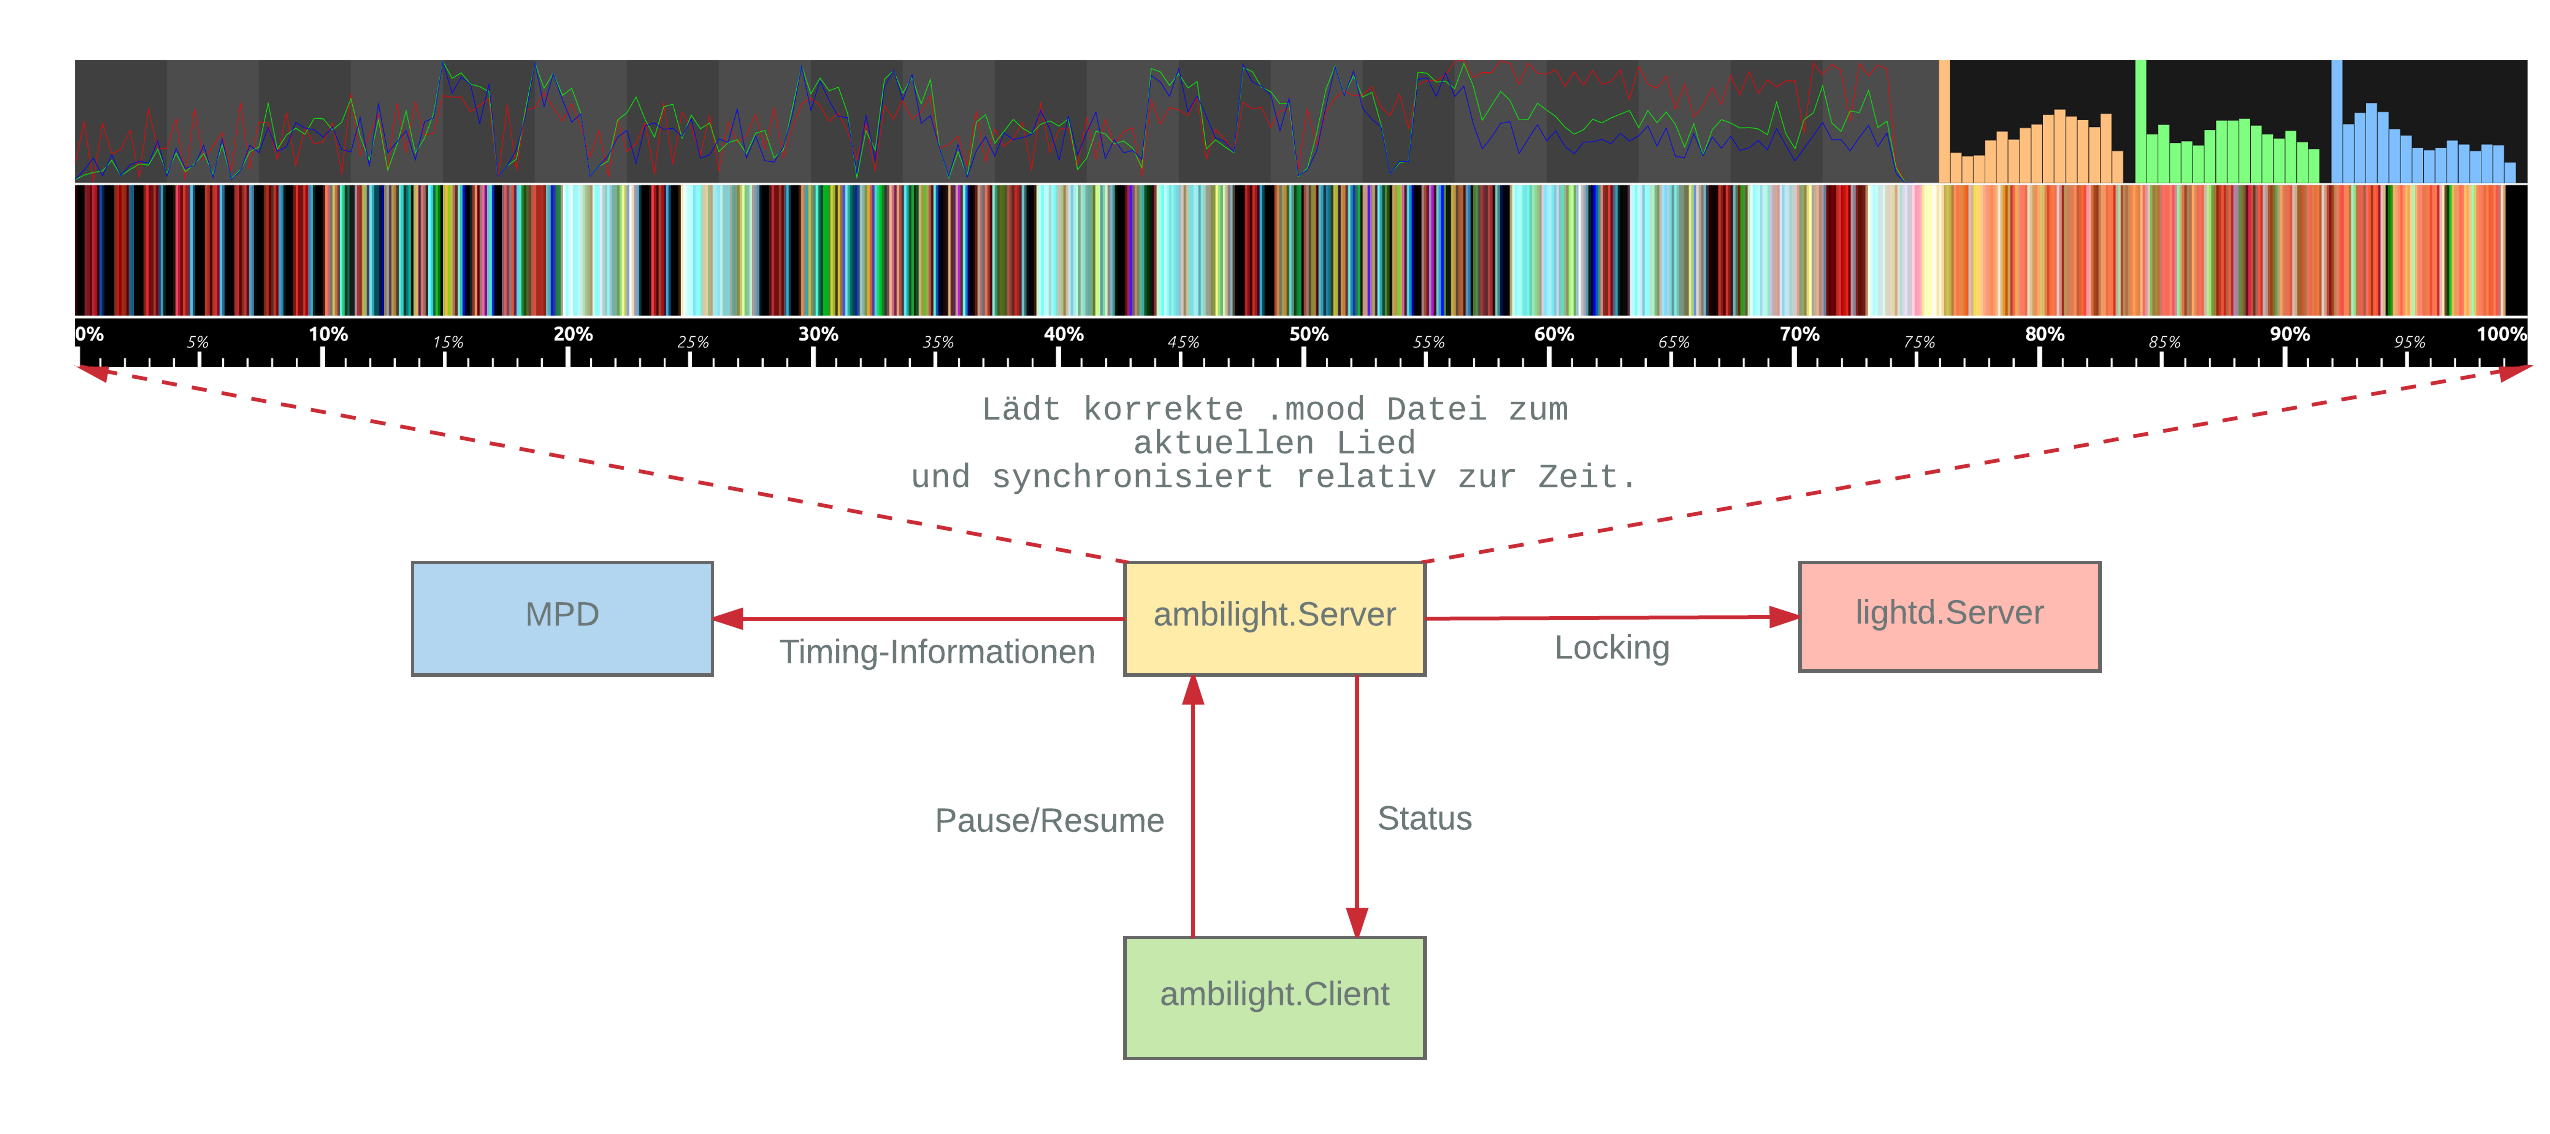
\includegraphics[width=1.0\textwidth]{images/eulenfunk-ambilight.png}
  \caption{}
  \label{eulenfunk-ambilight}
\end{figure}

\begin{itemize}
\tightlist
\item
  Synchronisation zur Musik via MPD-Client.
\item
  Datenhaltung in \enquote{mood} directory/update funktion.
\end{itemize}

\subsection{mpdinfo}\label{mpdinfo}

\subsection{ui}\label{ui}

\begin{itemize}
\tightlist
\item
  Windows (mehr dazu im Designteil)
\end{itemize}

\subsection{automount}\label{automount}

\begin{itemize}
\tightlist
\item
  udev regel erklären
\item
  Root und systemd problem
\end{itemize}

\begin{figure}[h!]
  \centering
  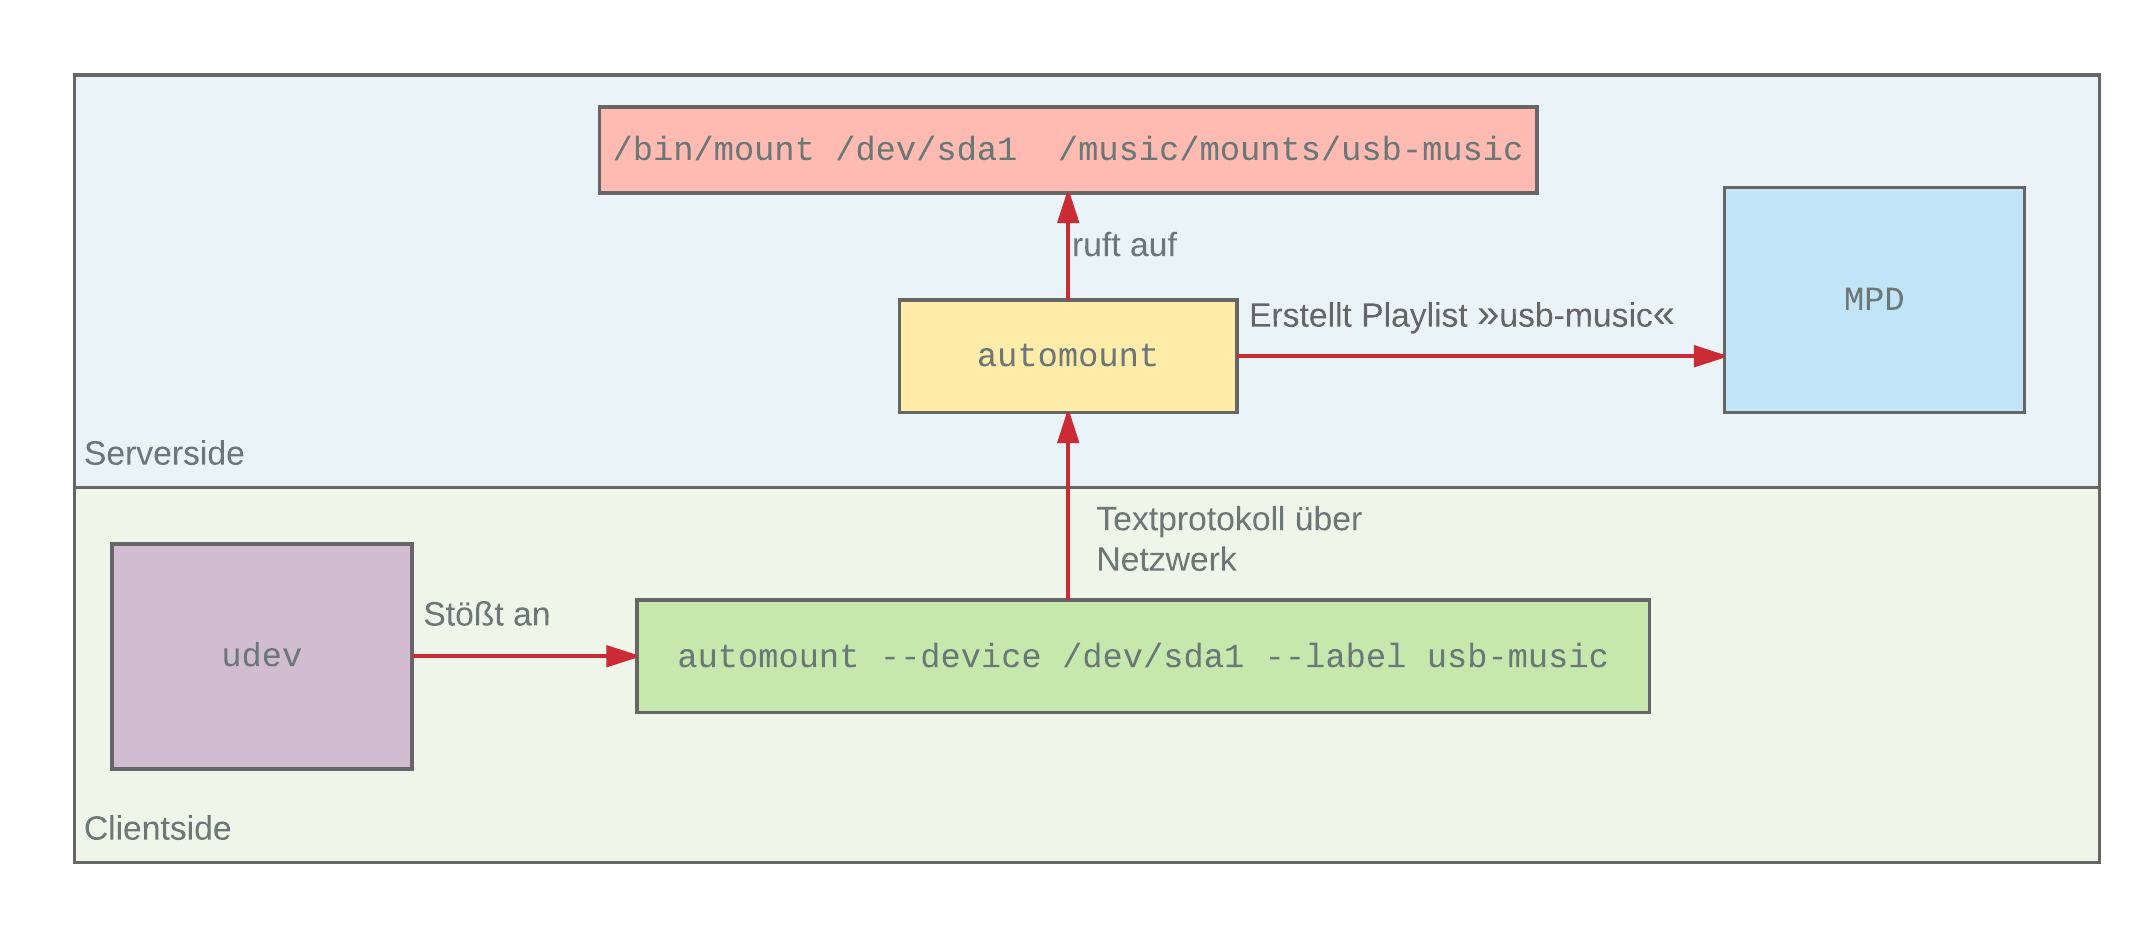
\includegraphics[width=1.0\textwidth]{images/eulenfunk-automount.png}
  \caption{}
  \label{eulenfunk-automount}
\end{figure}

\section{Einrichtung}\label{einrichtung}

\subsection{mpd und ympd}\label{mpd-und-ympd}

TODO: eigentliche mpd einrichrung.

\texttt{mpd} und \texttt{ympd} sind die einzigen Dienste die von außen
(ohne Authentifizierung) zugreifbar sind. Auch wenn \emph{Eulenfunk}
normal in einem abgesicherten WLAN hängt, wurde für die beiden Dienste
jeweils ein eigener Nutzer mit eingeschränkten Rechten und
\texttt{/bin/false} als Login--Shell angelegt.

\subsection{systemd}\label{systemd}

In Abbildung \ref{eulenfunk-systemd} ist schematisch der
Abhängigkeitsgraph der einzelnen Dienste gezeigt.

\begin{figure}[h!]
  \centering
  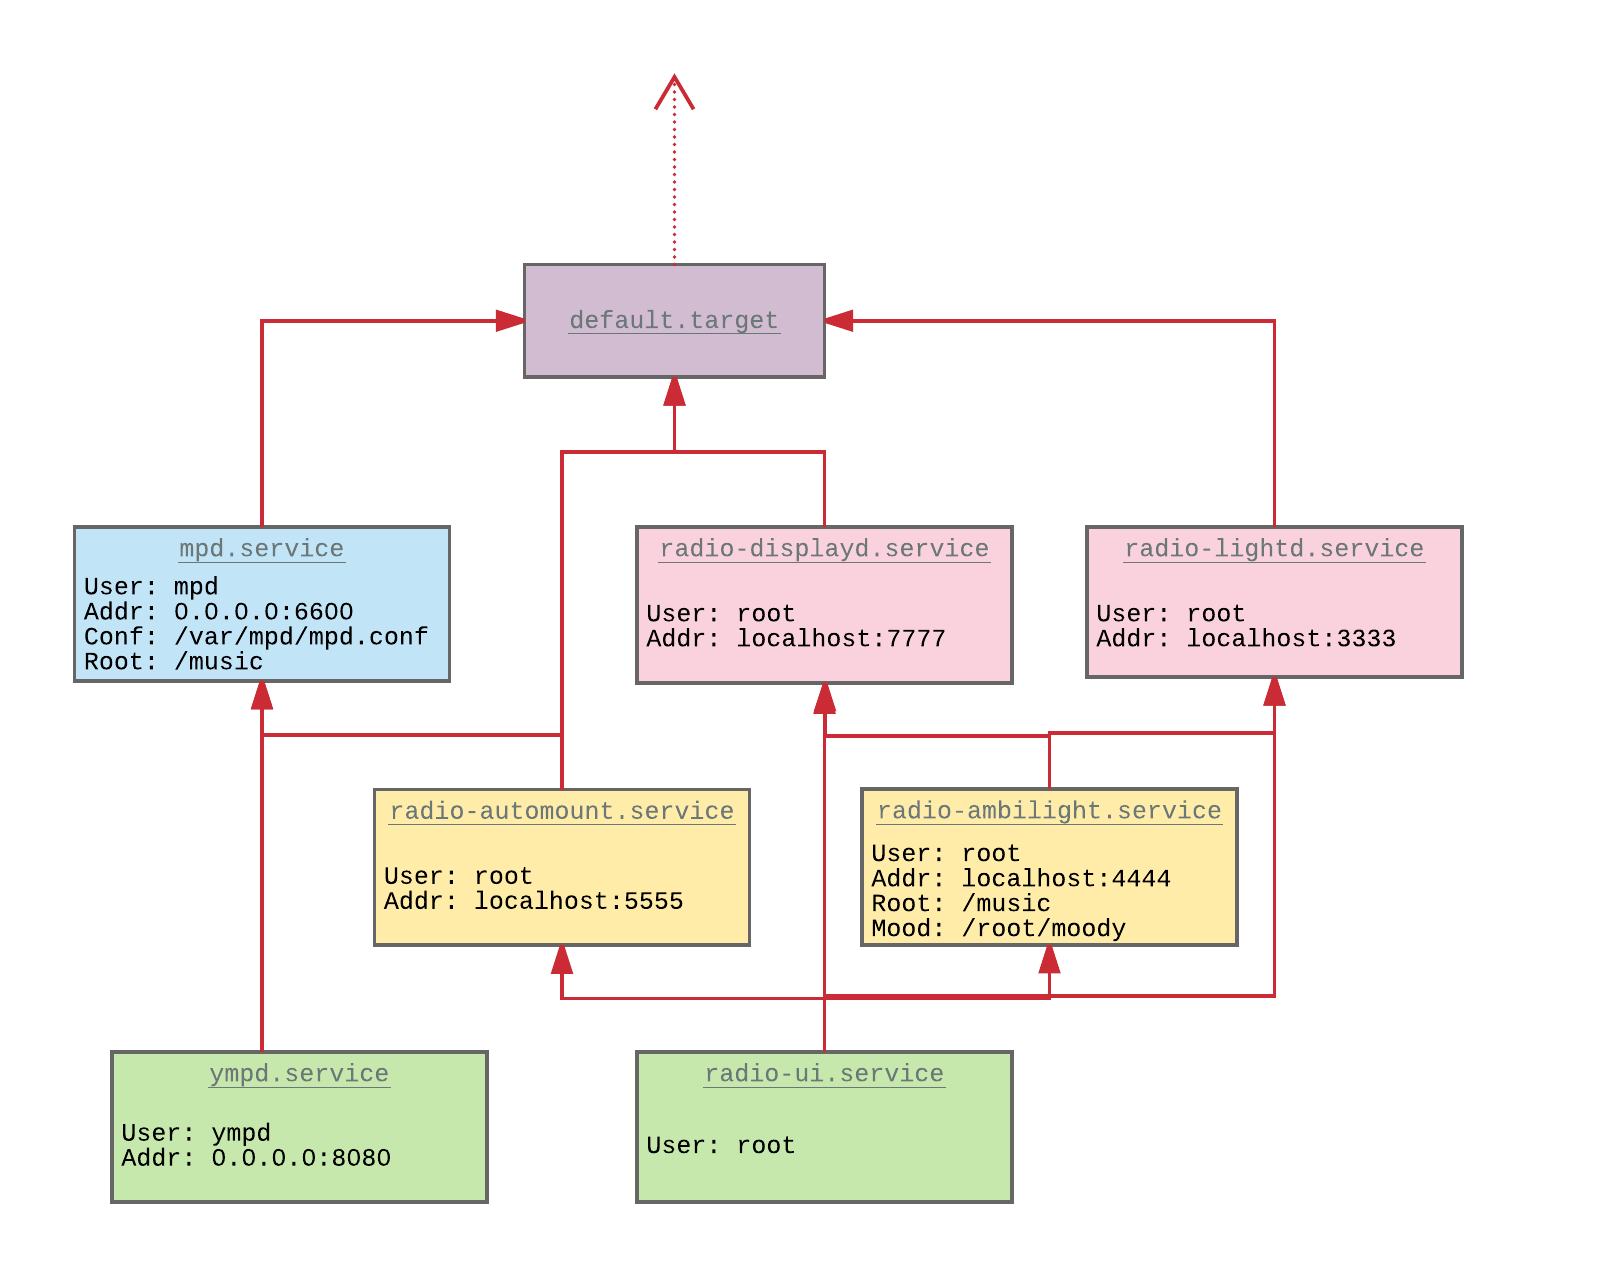
\includegraphics[width=0.9\textwidth]{images/eulenfunk-systemd.png}
  \caption{Abhängigkeits Graph beim Start der einzelnen Dienste}
  \label{eulenfunk-systemd}
\end{figure}

TODO: restart / restart-on-failure

\subsection{udev}\label{udev}

\subsection{sonstiges}\label{sonstiges}

Makefile

pstree

zeroconf

memory usage, cpu usage

godoc:

systemd boot plot

https://godoc.org/github.com/studentkittens/eulenfunk/display

\section{Wartung}\label{wartung}

ssh zugang

systemctl status/journalctl zum logging

\section{Fazit}\label{fazit}

cloc statistiken

probleme: re-mount, mpd brokenness.

\chapter{Zusammenfassung}\label{zusammenfassung}

\section{Ziel erreicht?}\label{ziel-erreicht}

Das selbstgesetzte Ziel --- mit möglichst wenig Aufwand ein
Internetradio auf Basis eines \emph{Raspberry Pi} zu entwickeln --- kann
durchaus als erfolgreich betrachtet werden.

\section{Erweiterungen und alternative
Ansätze}\label{erweiterungen-und-alternative-ansuxe4tze}

\subsection{Allgemein}\label{allgemein}

Der aktuelle Prototyp hat lediglich nur ein Potentiometer um die
Hintergrundbeleuchtung des LCD zu regeln. Ein anderer Ansatz wäre der
Einsatz eines Relais, welches es ermöglichen würde die
LCD--Hintergrundbeleuchtung Software--seitig ein-- und auszuschalten.

\subsection{Audio--Visualisierung}\label{audiovisualisierung}

Beim Projekt \emph{Eulenfunk} wird die Visualisierung von Musik aufgrund
der begrenzten Zeit und Hardwareressourcen des \emph{Raspberry Pi }über
eine vorberechnete Moodbar--Datei realisiert. Dieser Ansatz funktioniert
bei nicht live gestreamter Musik gut. Bei live gestreamter Musik könnte
für die Visualisierung eine Fast--Fourier--Transformation in Echtzeit
durchgeführt werden. Da jedoch die Ressourcen des \emph{Raspberry Pi}
sehr begrenzt sind, sollte hier auf die Verwendung einer
GPU--beschleunigten--FFT zurückgegriffen werden (vgl. {[}12{]}, Seite
657 ff.).

Ein alternativer Ansatz wäre auch die Realisierung einer
Musik--Visualisierung mittels Hardwarekomponenten. Ein möglicher Ansatz
aus Hardware--basierten Hochpass-- und Tiefpassfiltern in Form einer
Disco--Beleuchtung wird unter {[}6{]}, Seite 261 ff. beschrieben.

\subsection{Echtzeituhr}\label{echtzeituhr}

Der \emph{Raspberry Pi} besitzt keine Hardware--Uhr. Aufgrund der
Tatsache, dass es sich bei \emph{Eulenfunk} um ein Internetradio handelt
wurde auf eine Echtzeituhr (real time clock, RTC) verzichtet, da sich
die Uhr von \emph{Eulenfunk} aufgrund der permanenten Internetverbindung
mittels NTP\footnote{Network Time Protocol:
  \url{https://de.wikipedia.org/wiki/Network_Time_Protocol}} über das
Internet synchronisieren kann. Eine Erweiterung um eine Echtzeituhr wird
in {[}5{]}, Seite 145 ff. und {[}4{]}, Seite 77 ff. ausführlich
beschrieben.

\subsection{Fernbedienung}\label{fernbedienung}

Eine weitere Erweiterung wäre die Integration einer Fernbedienung. Diese
ließe sich relativ einfach mittels eines Infrarot--Sensors und
beispielsweise der \emph{lirc}--Bibliothek umsetzen. Siehe auch
{[}10{]}, Seite 190 ff. für weitere Informationen.

\subsection{Batteriebetrieb}\label{batteriebetrieb}

Da die Strom-- beziehungsweise Spannungsversorgung beim \emph{Raspberry
Pi} problematisch ist, wäre auch ein Batterie-- beziehungsweise
Akkubetrieb möglich. Eine einfache Schaltung für einen Batteriebetrieb
würde sich beispielsweise mit einem \emph{LM7805}--Spannungsregler oder
einem Abwärtswandler realisieren lassen ({[}3{]}, Seite 24 ff.).

\section{Mögliche Verbesserungen}\label{muxf6gliche-verbesserungen}

\subsection{Alpine Linux}\label{alpine-linux}

Die relativ junge Linux--Distribution \emph{Alpine Linux}\footnote{Alpine
  Linux für Raspberry Pi:
  \url{https://wiki.alpinelinux.org/wiki/Raspberry_Pi}} wäre eine
mögliche Verbesserung für den Einsatzzweck Internetradio. Diese
Distribution hat ihren Fokus auf Ressourceneffizienz und
Systemsicherheit. Ein weiterer Vorteil wäre der \texttt{diskless\ mode},
welcher das komplette Betriebssystem in den Arbeitsspeicher lädt. In
diesem Modus müssen Änderungen mit einem \emph{Alpine Local Backup
(lbu)}--Tool explizit auf die Festplatte geschrieben werden. Das hätte
den Vorteil, dass man die Abnutzung des Flash--Speichers, durch unnötige
Schreib/Lese--Vorgänge, minimieren würde.

\chapter*{Literaturverzeichnis}\label{literaturverzeichnis}
\addcontentsline{toc}{chapter}{Literaturverzeichnis}

\hypertarget{refs}{}
\hypertarget{ref-gay2014raspberry}{}
{[}1{]} W. Gay, \emph{Raspberry Pi Hardware Reference}. Apress, 2014.

\hypertarget{ref-richardson2014make}{}
{[}2{]} M. Richardson and S. Wallace, \emph{Make: Getting Started with
Raspberry Pi}. Maker Media, 2014.

\hypertarget{ref-gay2014mastering}{}
{[}3{]} W. Gay, \emph{Mastering the Raspberry Pi}. Apress, 2014.

\hypertarget{ref-gay2014experimenting}{}
{[}4{]} W. Gay, \emph{Experimenting with Raspberry Pi}. Apress, 2014.

\hypertarget{ref-horan2013practical}{}
{[}5{]} B. Horan, \emph{Practical Raspberry Pi}. Apress, 2013.

\hypertarget{ref-2014projekte}{}
{[}6{]} \emph{Projekte mit dem Raspberry Pi:}. mitp/bhv, 2014.

\hypertarget{ref-exploring}{}
{[}7{]} D. Molloy, in \emph{Exploring Raspberry Pi}, John Wiley \& Sons,
Inc., 2016.

\hypertarget{ref-suehle2014hacks}{}
{[}8{]} R. Suehle and T. Callaway, \emph{Hacks für Raspberry Pi}.
O'Reilly Verlag, 2014.

\hypertarget{ref-pietraszak2014buch}{}
{[}9{]} S. Pietraszak, \emph{Das Buch zu Raspberry Pi mit Linux}.
O'Reilly Verlag, 2014.

\hypertarget{ref-warner2013hacking}{}
{[}10{]} T. Warner, \emph{Hacking Raspberry Pi}. Pearson Education,
2013.

\hypertarget{ref-schmidt2014raspberry}{}
{[}11{]} M. Schmidt, \emph{Raspberry Pi: Einstieg - Optimierung -
Projekte}. Dpunkt.Verlag GmbH, 2014.

\hypertarget{ref-Sabarinath2015}{}
{[}12{]} S. Sabarinath, R. Shyam, C. Aneesh, R. Gandhiraj, and K. P.
Soman, ``Accelerated FFT Computation for GNU Radio Using GPU of
Raspberry Pi,'' in \emph{Computational intelligence in data mining -
volume 2: Proceedings of the international conference on cidm, 20-21
december 2014}, C. L. Jain, S. H. Behera, K. J. Mandal, and P. D.
Mohapatra, Eds. New Delhi: Springer India, 2015.

\end{document}
